
\documentclass[12pt,a4paper]{report}
% Packages for enhanced functionality
\usepackage[utf8]{inputenc}
\usepackage[T1]{fontenc}
\usepackage{graphicx} % For including images
\usepackage{amsmath}  % For mathematical equations
\usepackage{geometry} % For page layout
\usepackage{hyperref} % For clickable links and references
\usepackage{fancyhdr} % For custom headers and footers
\usepackage{titlesec} % For section title formatting
\usepackage{float}
\usepackage{circuitikz}
\usepackage{caption}
\usepackage{siunitx}
\usepackage{amsmath}
\usepackage{subcaption}
\usepackage{booktabs}
\hypersetup{
    colorlinks=true,  % Enable colored text links
    linkcolor=orange,    % Internal links (sections, table of contents, etc.)
    urlcolor=orange,     % External URLs
    citecolor=orange,    % Citations
    pdfborder={0 0 0} % Remove ugly default borders
}
\begin{document}
\title{\textbf{EE1060 Quiz 3}\\
\LARGE{\textbf{Response of a Series RL Circuit to a Square Wave Input}}

\author{ Arjun Pavanje(EE24BTECH11005)\\M.B.S.Aravind (EE24BTECH11038)\\Shiny Diavajna.P (EE24BTECH11058)\\Homa Harshitha.V (EE24BTECH11062)\\Shivam Shilvant (EE24BTECH11057)\\Pranay Kumar.B (EE24BTECH11011)}

\begin{center}
	%\Large{Arjun Pavanje(EE24BTECH11005)\\M.B.S.Aravind (EE24BTECH11038)\\Shiny Diavajna.P (EE24BTECH11058)\\Homa Harshitha.V (EE24BTECH11062)\\Shivam Shilvant (EE24BTECH11057)\\Pranay Kumar.B (EE24BTECH11011)}\\
\end{center}
\vspace{30pt}
\begin{figure}[ht]
	\centering
	
\includegraphics[width = 100pt]{.logo/logo.png}\\
\end{figure}
\begin{center}
	Bachelor of Technology\\
	\vspace{10pt}
	Department of Electrical Engineering\\
\end{center}
}
\maketitle

% Title page settings
%\title{
%    \vspace{2in}
%    \Huge{\textbf{Response of a Series RL Circuit to a Square Wave Input}} \\
%    \Large{} \\
%    \vspace{1in}
%    \vspace{1in}
%    \Large{Arjun Pavanje(EE24BTECH11005)\\M.B.S.Aravind (EE24BTECH11038)\\Shiny Diavajna.P (EE24BTECH11058)\\Homa Harshitha.V (EE24BTECH11062)\\Shivam Shilvant (EE24BTECH11057)\\Pranay Kumar.B (EE24BTECH11011)}\\
%    \Large{Date: \today}
%}
%\author{}
%\date{}
%% Section title formatting
%\titleformat{\chapter}[hang]{\Huge\bfseries}{\thechapter.}{20pt}{}
%\titleformat{\section}[hang]{\Large\bfseries}{\thesection}{12pt}{}
%\titleformat{\subsection}[hang]{\large\bfseries}{\thesubsection}{10pt}{}
%\begin{document}
%% Title page
%\maketitle

% Table of Contents
\tableofcontents
\chapter{Introduction}
The goal of this report is to analyze the response of a series $RL$ circuit to a square wave input using numerical methods and compare to the result obtained using fourier series.


\begin{figure}[H]
\centering
\begin{tikzpicture}[scale=0.8]
\draw[->] (-0.5,0) -- (8,0) node[right] {$t$};
\draw[->] (0,-0.5) -- (0,3) node[above] {$v(t)$};
\draw (0,0) -- (0,2);
\draw (0,2) -- (2,2);
\draw (2,2) -- (2,0);
\draw (2,0) -- (4,0);
\draw (4,0) -- (4,2);
\draw (4,2) -- (6,2);
\draw (6,2) -- (6,0);
\draw (6,0) -- (8,0);
\draw[dashed] (0,2) -- (8,2);
\draw (2,-0.1) -- (2,0.1) node[below] {$\alpha T$};
\draw (4,-0.1) -- (4,0.1) node[below] {$T$};
\draw (6,-0.1) -- (6,0.1) node[below] {$(1+\alpha)T$};
\draw (8,-0.1) -- (8,0.1) node[below] {$2T$};
\draw (0,2) node[left] {$10$};
\end{tikzpicture}
\caption{Square wave with a duty ratio $\alpha$}
\end{figure}
Circuit, 
\begin{figure}[!ht]
\centering
\resizebox{0.5\textwidth}{!}{%
\begin{circuitikz}
\tikzstyle{every node}=[font=\normalsize]
\draw (6.25,13) to[R,l={ \normalsize $R$}] (10,13);
\draw (10,13) to[L,l={ \normalsize $L$} ] (10,9.25);
\draw (6.25,13) to[square voltage source, sources/symbol/rotate=auto,l={ \normalsize $V_{sq}$}] (6.25,9.25);
\draw (6.25,9.25) to[short] (10,9.25);
\draw (10,13) to[short, -o] (11.25,13) ;
\draw (10,9.25) to[short, -o] (11.25,9.25) ;
\end{circuitikz}
}%
\label{fig:my_label}
\end{figure}


\chapter{Governing Differential Equation}
\section{Current response}
The behavior of the RL circuit is governed by:
\begin{equation}
L\frac{di}{dt} + Ri = v(t)
\end{equation}


Where $v(t)$ is the square wave input voltage defined as:
\begin{equation}
v(t) = 
\begin{cases}
10, & 0 < t < \alpha T \\
0, & \alpha T < t < T
\end{cases}
\end{equation}

Rearranging to standard form:
\begin{equation}
\frac{di}{dt} = \frac{v(t) - Ri}{L}
\end{equation}
\section{Voltage across inductor}
The voltage across inductor is given by
\begin{align}
    V_L=L\frac{di}{dt}
\end{align}
\section{Voltage across Resistor}
The voltage across resistor is given by
\begin{align}
    V_R=Ri
\end{align}
\chapter{Numerical Methods}
Code used to plot all numerical methods, fourier series. Run the code to see each numerical method at different values of $\tau, L, \alpha, T$ and to compare the numerical methods. \url{https://github.com/ArjunPavanje/EE1060/blob/main/Quiz3/codes/numerical_methods.py}
\section{Forward Euler Method}
The Forward Euler method is an explicit first-order numerical method for solving ordinary differential equations. For our RL circuit, the update equation is:

\begin{equation}
i_{n+1} = i_n + h \cdot \frac{v(t_n) - Ri_n}{L}
\end{equation}

Where $h$ is the step size and $i_n$ is the current at time step $n$.

\textbf{Derivation:}
Starting with the differential equation:
\begin{equation}
\frac{di}{dt} = \frac{v(t) - Ri}{L}
\end{equation}

Using the forward difference approximation:
\begin{equation}
\frac{di}{dt} \approx \frac{i_{n+1} - i_n}{h}
\end{equation}

Substituting this into the differential equation:
\begin{equation}
\frac{i_{n+1} - i_n}{h} = \frac{v(t_n) - Ri_n}{L}
\end{equation}

Solving for $i_{n+1}$:
\begin{equation}
i_{n+1} = i_n + h \cdot \frac{v(t_n) - Ri_n}{L}
\end{equation}

\begin{figure}[h!]
	\centering
	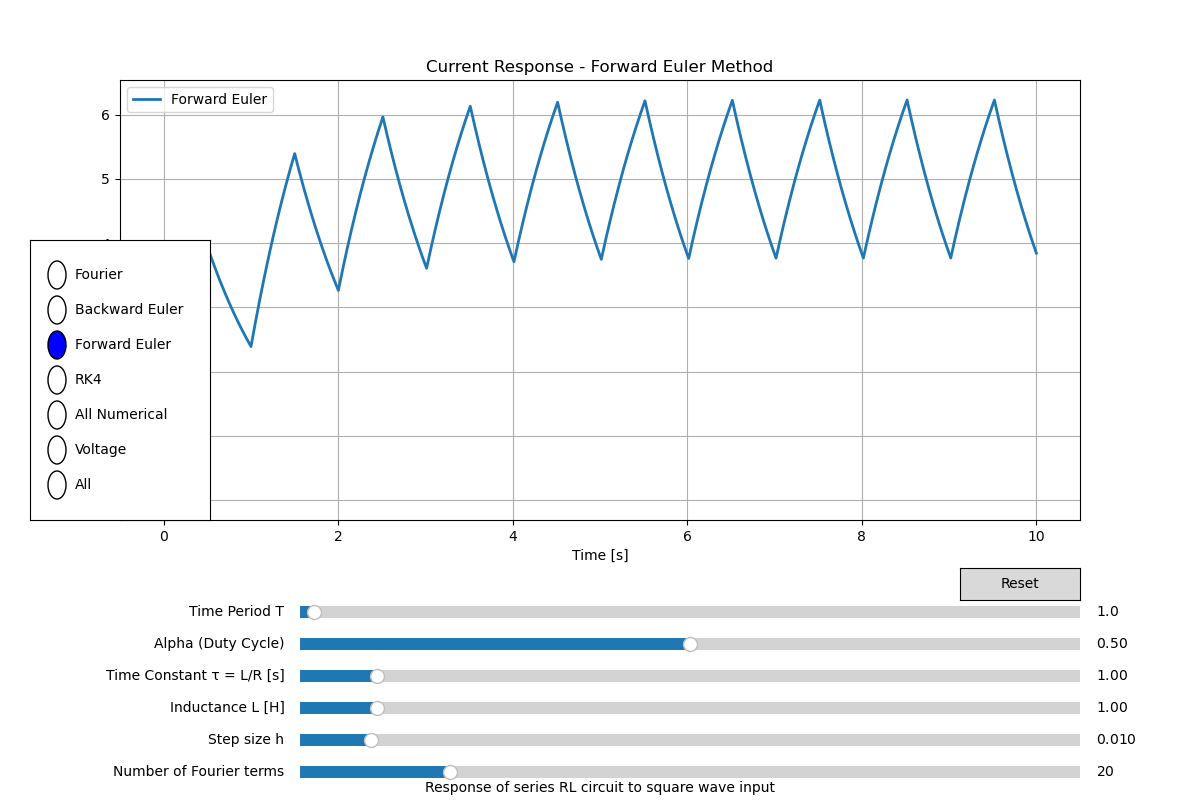
\includegraphics[scale=0.5]{figs/ForwardEuler-numerical.png}
\end{figure}



\section{Backward Euler Method}
The Backward Euler method is an implicit first-order numerical method. For our RL circuit, the update equation is:

\begin{equation}
i_{n+1} = i_n + h \cdot \frac{v(t_{n+1}) - Ri_{n+1}}{L}
\end{equation}

\textbf{Derivation:}
Starting with the differential equation:
\begin{equation}
\frac{di}{dt} = \frac{v(t) - Ri}{L}
\end{equation}

Using the backward difference approximation:
\begin{equation}
\frac{di}{dt} \approx \frac{i_{n+1} - i_n}{h}
\end{equation}

Substituting this into the differential equation:
\begin{equation}
\frac{i_{n+1} - i_n}{h} = \frac{v(t_{n+1}) - Ri_{n+1}}{L}
\end{equation}

Solving for $i_{n+1}$:
\begin{equation}
i_{n+1} = \frac{Li_n + hv(t_{n+1})}{L + hR} = \frac{i_n\tau + hv(t_{n+1})}{\tau + h}
\end{equation}

Where $\tau = \frac{L}{R}$ is the time constant of the circuit.

\begin{figure}[h!]
	\centering
	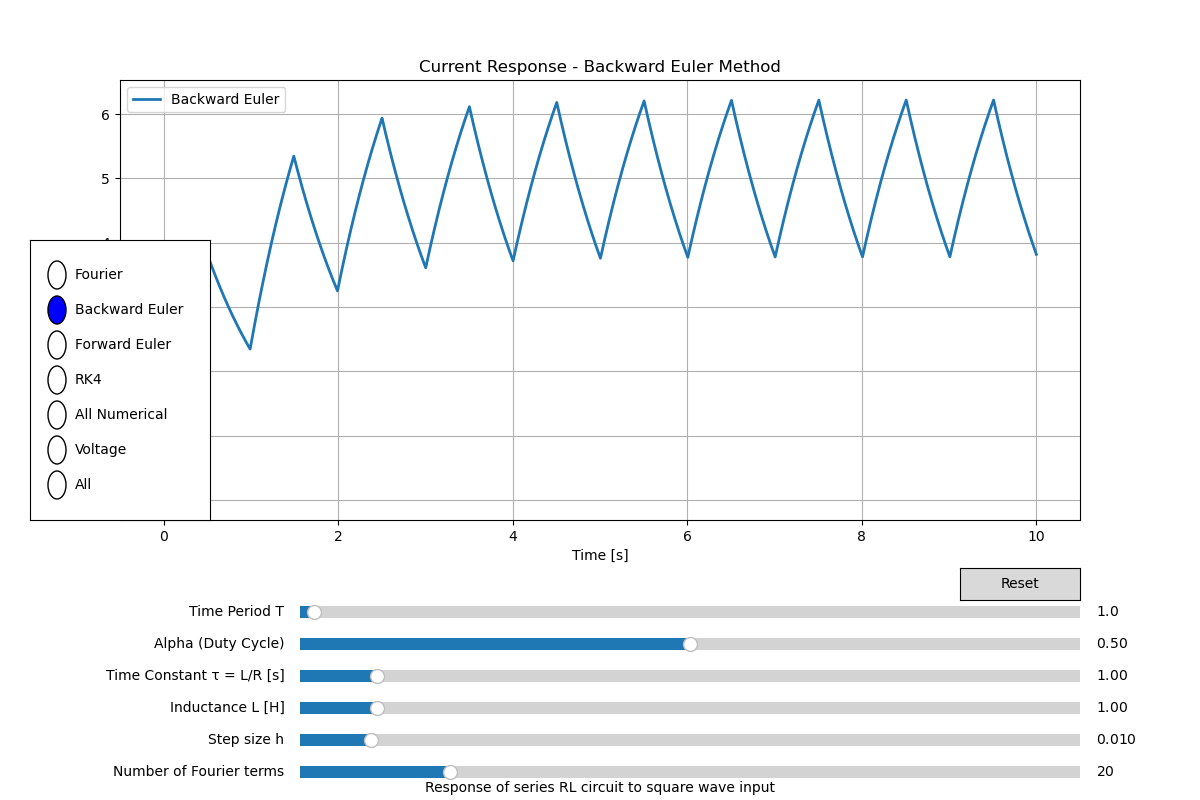
\includegraphics[scale=0.5]{figs/BackwardEuler-numerical.png}
        \end{figure}

\section{Runge-Kutta 4th Order Method (RK4)}
The RK4 method is a fourth-order method for numerically solving ordinary differential equations. For our RL circuit, the update equation is:

\begin{equation}
i_{n+1} = i_n + \frac{1}{6}(k_1 + 2k_2 + 2k_3 + k_4)
\end{equation}

\textbf{Derivation:}
For the differential equation $\frac{di}{dt} = f(t, i) = \frac{v(t) - Ri}{L}$, the RK4 method computes:

\begin{align}
k_1 &= h \cdot f(t_n, i_n) = h \cdot \frac{v(t_n) - Ri_n}{L} \\
k_2 &= h \cdot f(t_n + \frac{h}{2}, i_n + \frac{k_1}{2}) = h \cdot \frac{v(t_n + \frac{h}{2}) - R(i_n + \frac{k_1}{2})}{L} \\
k_3 &= h \cdot f(t_n + \frac{h}{2}, i_n + \frac{k_2}{2}) = h \cdot \frac{v(t_n + \frac{h}{2}) - R(i_n + \frac{k_2}{2})}{L} \\
k_4 &= h \cdot f(t_n + h, i_n + k_3) = h \cdot \frac{v(t_n + h) - R(i_n + k_3)}{L}
\end{align}

The current at the next time step is then:
\begin{equation}
i_{n+1} = i_n + \frac{1}{6}(k_1 + 2k_2 + 2k_3 + k_4)
\end{equation}

\begin{figure}[h!]
	\centering
	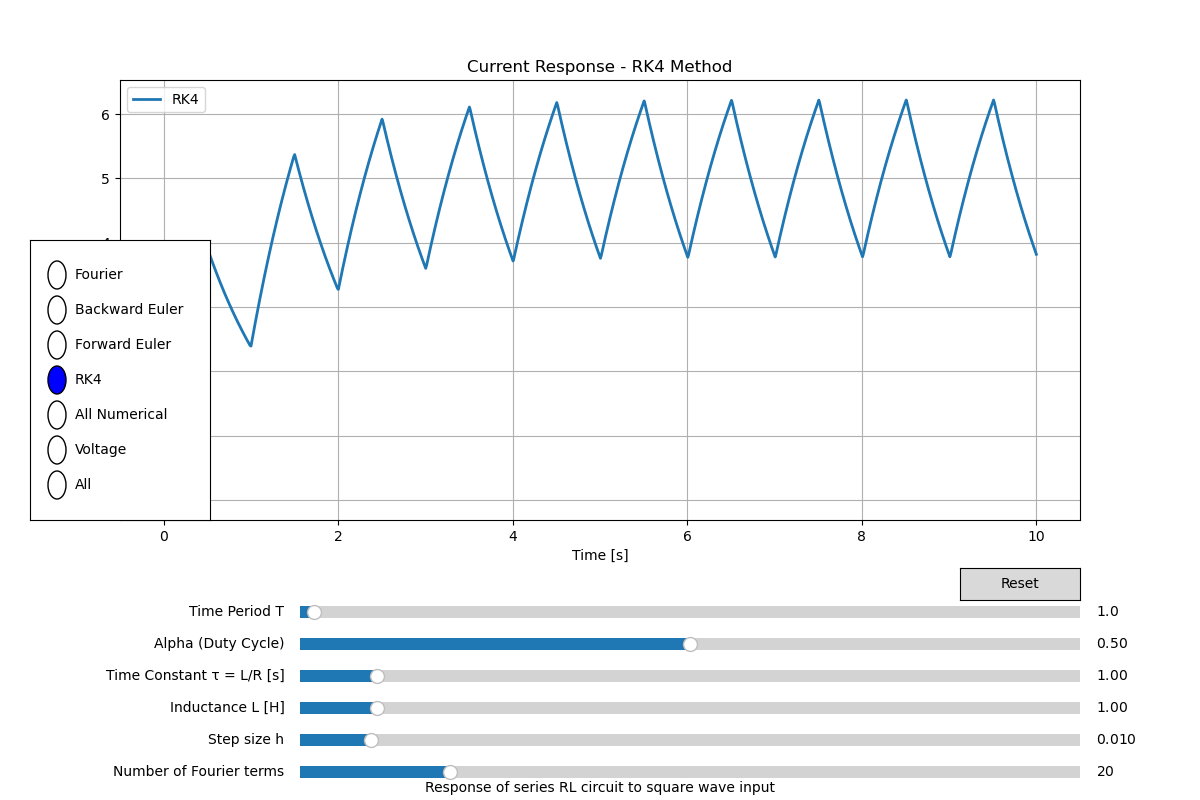
\includegraphics[scale=0.5]{figs/RK4-numerical.png}
\end{figure}
Plots for voltage across inductor by various numerical methods can be found using the followning python code, \url{https://github.com/ArjunPavanje/EE1060/blob/main/Quiz3/codes/voltage.py}
\chapter{Analytical Method: Fourier Series}
\section{Fourier Series}
The square wave voltage can be represented using Fourier series:

\begin{equation}
v(t) = a_0 + \sum_{n=1}^{\infty}\left[a_n\cos\left(\frac{2\pi nt}{T}\right) + b_n\sin\left(\frac{2\pi nt}{T}\right)\right]
\end{equation}

\textbf{Derivation of Fourier Coefficients:}
For the square wave defined as:
\begin{equation}
v(t) = 
\begin{cases}
10, & 0 < t < \alpha T \\
0, & \alpha T < t < T
\end{cases}
\end{equation}

The Fourier coefficients are:

1. DC component $a_0$:
\begin{align}
a_0 &= \frac{1}{T}\int_{0}^{T} v(t)dt \\
&= \frac{1}{T}\left[\int_{0}^{\alpha T} 10 dt + \int_{\alpha T}^{T} 0 dt\right] \\
&= \frac{10\alpha T}{T} = 10\alpha
\end{align}

2. Cosine coefficients $a_n$:
\begin{align}
a_n &= \frac{2}{T}\int_{0}^{T} v(t)\cos\left(\frac{2\pi nt}{T}\right)dt \\
&= \frac{2}{T}\int_{0}^{\alpha T} 10\cos\left(\frac{2\pi nt}{T}\right)dt \\
&= \frac{20}{T} \cdot \frac{T}{2\pi n}[\sin(2\pi n\alpha) - \sin(0)] \\
&= \frac{10}{\pi n}\sin(2\pi n\alpha)
\end{align}

3. Sine coefficients $b_n$:
\begin{align}
b_n &= \frac{2}{T}\int_{0}^{T} v(t)\sin\left(\frac{2\pi nt}{T}\right)dt \\
&= \frac{2}{T}\int_{0}^{\alpha T} 10\sin\left(\frac{2\pi nt}{T}\right)dt \\
&= \frac{2 \cdot 10}{T}\left[\frac{-T}{2\pi n}\cos\left(\frac{2\pi nt}{T}\right)\right]_{0}^{\alpha T} \\
&= \frac{-20}{2\pi n}[\cos(2\pi n\alpha) - \cos(0)] \\
&= \frac{10}{\pi n}[1 - \cos(2\pi n\alpha)]
\end{align}

Therefore, the Fourier series for $v(t)$ is:
\begin{equation}
v(t) = 10\alpha + \sum_{n=1}^{\infty}\left(\frac{10}{\pi n}\sin(2\pi n\alpha)\cos\left(\frac{2\pi nt}{T}\right) + \frac{10}{\pi n}[1-\cos(2\pi n\alpha)]\sin\left(\frac{2\pi nt}{T}\right)\right)
\end{equation}

\textbf{Calculating  $I(t)$}\\
Given differential equation is\\
\begin{align}
L\frac{di}{dt} + iR = 10\alpha + \sum_{n=1}^{\infty}\left(\frac{10}{n\pi}\sin(2\pi n\alpha)\cos\left(\frac{2\pi n t}{T}\right) + \frac{10}{n\pi}(1-\cos(2\pi n\alpha))\sin\left(\frac{2\pi nt}{T}\right)\right)
\end{align}


Since the system is linear, we solve for each harmonic component separately:\\
Assume a solution of the form:\\
\begin{align}
I_n = A_n\cos(n\omega_0 t) + B_n\sin(n\omega_0 t). \tag{0.18}
\end{align}

Substituting into the differential equation and solving for $A_{n}$ and $B_{n}$ we obtain:\
\begin{align}
A_n = \frac{b_nR}{R^2 + (n\omega_0L)^2}, \quad B_n = \frac{b_n n\omega_0 L}{R^2 + (n\omega_0L)^2}. \tag{0.19}
\end{align}

Thus, the total current response is given by:\\
\begin{align*}
I(t) = \frac{10\alpha}{R}\left(1-e^{-\frac{R}{L}t}\right) + \sum_{n=1}^{\infty}\frac{10}{n\pi}\sin(2\pi \alpha n)\left[\frac{R\cos(n\omega_0t) + n\omega_0L\sin(n\omega_0t)}{R^2 + L^2(n\omega_0)^2} - \right. \\
\left. \frac{R}{R^2 + L^2(n\omega_0)^2}e^{-\frac{R}{L}t}\right] 
+ \sum_{n=1}^{\infty}\frac{10}{n\pi}(1-\cos(2\pi \alpha n))\left[\frac{R\sin(n\omega_0t) - Ln\omega_0\cos(n\omega_0t)}{R^2 + L^2(n\omega_0)^2} + \right. \\
\left. \frac{n\omega_0L}{R^2 + L^2(n\omega_0)^2}e^{-\frac{R}{L}t}\right] \tag{0.21}
\end{align*}
\section{Fourier Spectrum of $ V(t) $}

The given Fourier series is:

\begin{align}
V(t) = 10\alpha + \sum_{n=1}^{\infty} \left[ \frac{10}{\pi n} \sin(2\pi n \alpha) \cos\left( \frac{2\pi n t}{T} \right) + \frac{10}{\pi n} (1 - \cos(2\pi n \alpha)) \sin\left( \frac{2\pi n t}{T} \right) \right].
\end{align}

\subsection{Fourier Coefficients}

A Fourier series is expressed as:

\begin{align}
V(t) = A_0 + \sum_{n=1}^{\infty} A_n \cos\left( \frac{2\pi n t}{T} \right) + B_n \sin\left( \frac{2\pi n t}{T} \right).
\end{align}

From the given equation, we identify:

\begin{align}
A_0 = 10\alpha,
\end{align}

\begin{align}
A_n = \frac{10}{\pi n} \sin(2\pi n \alpha),
\end{align}

\begin{align}
B_n = \frac{10}{\pi n} (1 - \cos(2\pi n \alpha)).
\end{align}

\subsection{Amplitude Spectrum}

The amplitude of each frequency component is given by:

\begin{align}
C_n = \sqrt{A_n^2 + B_n^2}.
\end{align}

Substituting $ A_n $ and $ B_n $:

\begin{align}
C_n = \frac{10}{\pi n} \sqrt{\sin^2(2\pi n \alpha) + (1 - \cos(2\pi n \alpha))^2}.
\end{align}

Using the identity $ 1 - \cos x = 2 \sin^2(x/2) $:

\begin{align}
C_n = \frac{10}{\pi n} \sqrt{2 - 2\cos(2\pi n \alpha)}.
\end{align}

Since $ 1 - \cos x = 2 \sin^2(x/2) $, we simplify:

\begin{align}
C_n = \left|{{\frac{10}{\pi n} \cdot 2 \sin \left( \pi n \alpha \right)}}\right|.
\end{align}

Thus, the amplitude spectrum is:

\begin{align}
C_n = \left|{\frac{20}{\pi n} \sin(\pi n \alpha)}\right|.
\end{align}

\subsection{Phase Spectrum}

The phase $ \phi_n $ is given by:

\begin{align}
\phi_n = -\tan^{-1} \left( \frac{B_n}{A_n} \right).
\end{align}

Substituting $ A_n $ and $ B_n $:

\begin{align}
\phi_n = -\tan^{-1} \left( \frac{1 - \cos(2\pi n \alpha)}{\sin(2\pi n \alpha)} \right).
\end{align}

Using the identity $ 1 - \cos x = 2 \sin^2(x/2) $, we get:

\begin{align}
\phi_n = -\tan^{-1} \left( \frac{\sin^2 (\pi n \alpha)}{\sin (\pi n \alpha) \cos (\pi n \alpha)} \right).
\end{align}

Simplifying:

\begin{align}
\phi_n = -\tan^{-1} \left( \frac{\sin (\pi n \alpha)}{\cos (\pi n \alpha)} \right).
\end{align}

\subsection{Final Fourier Spectrum}

\begin{align}
C_n = \left|\frac{20}{\pi n} \sin(\pi n \alpha)\right|, \quad \phi_n = -\tan^{-1} \left(\tan (\pi n \alpha)\right).
\end{align}
To visually see the variation of spectrum with variation with $\alpha$, run the following code, \url{https://github.com/ArjunPavanje/EE1060/blob/main/Quiz3/codes/voltage_spectrum.py}

\begin{figure}[h!]
    \centering
    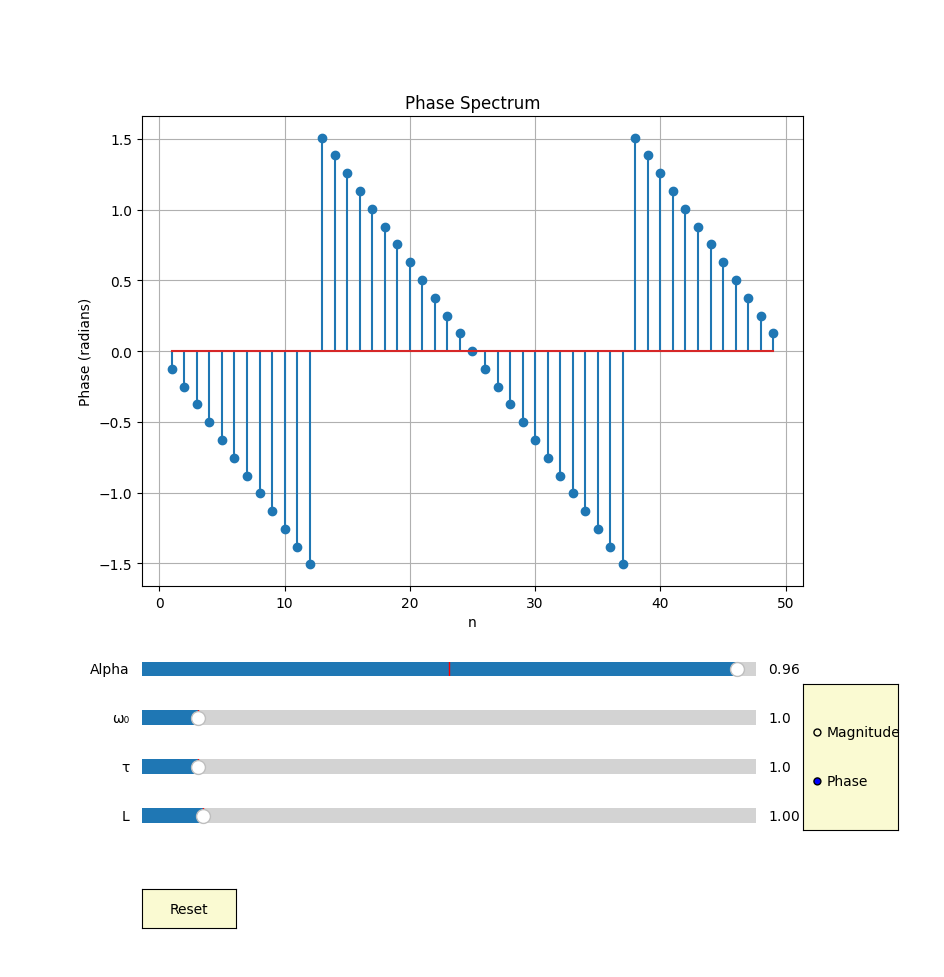
\includegraphics[width=0.7\linewidth]{figs/phase_spectrum.png}
    \label{fig:enter-label}
\end{figure}
\begin{figure}[h!]
    \centering
    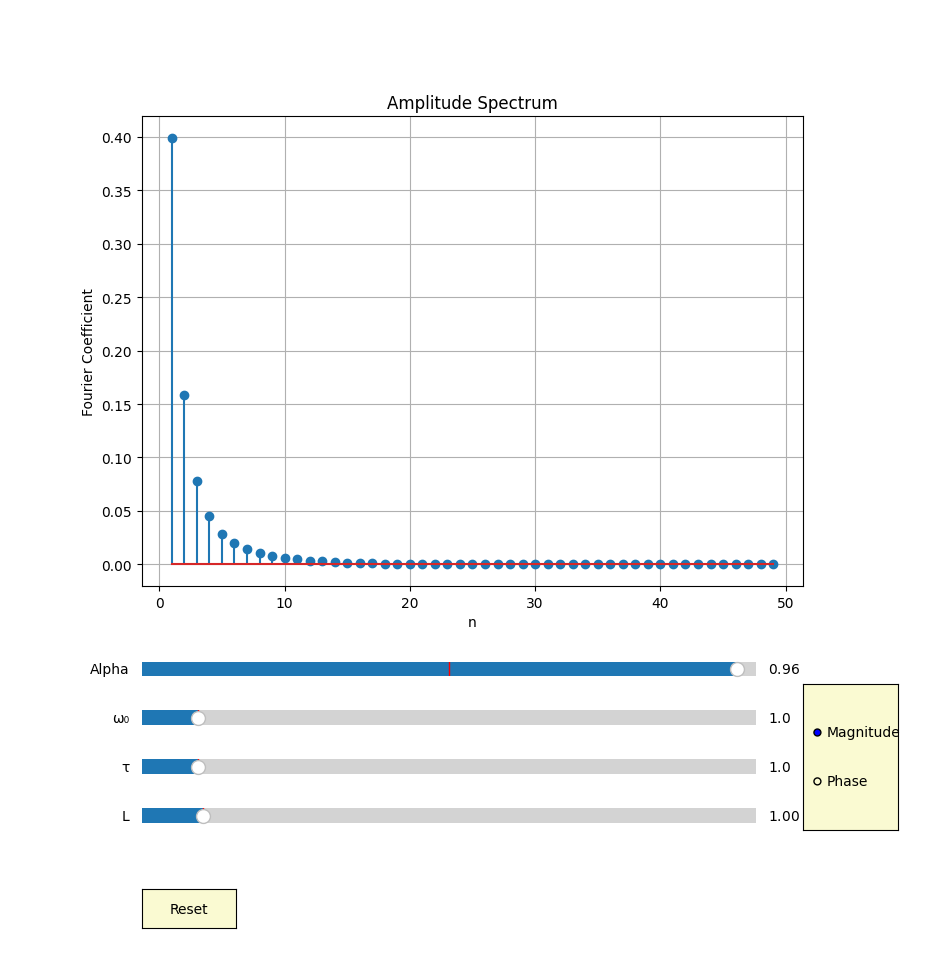
\includegraphics[width=1\linewidth]{figs/amplitude_spectrum.png}
    \label{fig:enter-label}
\end{figure}
This represents the amplitude and phase spectrum of the given Fourier series.

\newpage


\section{Convergence Behavior}

According to the Fourier Convergence Theorem, the Fourier series of a function $ f(t) $ converges to:
\begin{enumerate}
    \item The function value $ f(t) $ at all points where $ f(t) $ is continuous.
    \item The average of the left and right limits at points of discontinuity:
    \begin{align}
    \frac{1}{2} \left[ f(t^+) + f(t^-) \right].
    \end{align}
\end{enumerate}

\subsection{Conditions for Convergence}

For a Fourier series to converge properly, the function must satisfy certain conditions, known as Dirichlet's conditions:

\begin{enumerate}
    \item \textbf{Absolute Integrability:}  
    The function $ f(t) $ must be absolutely integrable over one period, which means that the integral of its absolute value over one period must be finite:
    \begin{align}
    \int_{T} |f(t)| dt < \infty.
    \end{align}
    This condition ensures that the function does not grow too large, which could prevent the Fourier series from converging.

    \item \textbf{Finite Number of Discontinuities:}  
    The function $ f(t) $ must have only a finite number of discontinuities in any finite interval.  
    If the function has an infinite number of discontinuities, the Fourier series may not converge properly.

    \item \textbf{Finite Number of Maxima and Minima:}  
    The function $ f(t) $ must have only a finite number of maxima and minima in any finite interval.  
    This prevents excessive oscillations, which could disrupt the convergence of the Fourier series.

    \item \textbf{Piecewise Continuity:}  
    The function $ f(t) $ must be piecewise continuous over its domain.  
    A function is said to be piecewise continuous if it can be divided into a finite number of subintervals where it is continuous, except for a finite number of jump discontinuities.

    \item \textbf{Convergence at Discontinuities:}  
    If $ f(t) $ has a discontinuity at $ t = t_0 $, then the Fourier series converges to the average of the left-hand and right-hand limits:
    \begin{align}
    f_{\text{Fourier}}(t_0) = \frac{1}{2} \left[ f(t_0^+) + f(t_0^-) \right].
    \end{align}
    This explains why, for functions with discontinuities, the Fourier series does not perfectly match the function but instead gives an approximation in the form of an average.

\end{enumerate}

\subsection{Gibbs Phenomenon: Overshoot at Discontinuities}

When a Fourier series approximates a function that has a jump discontinuity, an interesting effect known as the Gibbs phenomenon occurs. This phenomenon is characterized by:

\begin{enumerate}
    \item An overshoot near the discontinuity, which is approximately 9\% of the jump size.
    \item Persistent oscillations near the discontinuity, which do not disappear even if more terms are included in the Fourier series.
    \item The oscillations become narrower as more terms are added, meaning the deviation from the true function is localized near the discontinuity. However, the peak overshoot remains unchanged.
\end{enumerate}

Mathematically, for a Fourier series $ S_N(t) $ approximating a function with a jump discontinuity at $ t_0 $, the maximum deviation from the true function satisfies:
\begin{align}
\lim_{N \to \infty} \max |S_N(t) - f(t)| \approx 1.09 \times \frac{\text{Jump Size}}{2}.
\end{align}
This means that no matter how many terms we take, the Fourier series will always have an overshoot near discontinuities.
\subsection{Verification of Dirichlet’s Conditions and Gibbs Phenomenon}

The square wave function is defined as:

\begin{align}
f(t) =
\begin{cases}
A, & 0 < t < \alpha T \\
0, & \alpha T < t < T
\end{cases}
\end{align}

and is periodic with period $ T $. We verify Dirichlet’s conditions:

\begin{itemize}
    \item \textbf{Absolute Integrability:} The integral over one period is finite:
    \begin{align}
    \int_0^T |f(t)| dt = A \alpha T < \infty.
    \end{align}
    \item \textbf{Finite Discontinuities:} The function has two jump discontinuities at $ t = 0 $ and $ t = \alpha T $.
    \item \textbf{Finite Extrema:} The function has one maximum at $ A $ and one minimum at $ 0 $, satisfying the condition.
    \item \textbf{Piecewise Continuity:} The function is continuous except at a finite number of discontinuities.
\end{itemize}

Since all Dirichlet conditions are satisfied, the Fourier series converges. However, near discontinuities, the series overshoots by approximately $ 9\% $ of the jump due to Gibbs phenomenon, causing oscillations that persist regardless of the number of terms.


\subsection{Application to a Square Wave}

A square wave is a periodic function that alternates between two values, typically $ A $ and $ 0 $, with sharp transitions at certain points. These transitions are jump discontinuities. 

At points of discontinuity, such as $ t = 0 $ and $ t = \alpha T $, the Fourier series does not converge exactly to $ A $ or $ 0 $, but instead to:
\begin{align}
\frac{1}{2} \left( A + 0 \right) = \frac{A}{2}.
\end{align}
This follows from the general property that at a discontinuity, the Fourier series converges to the average of the left-hand and right-hand limits. However, due to Gibbs phenomenon, the Fourier series exhibits an overshoot near these discontinuities, causing oscillations that cannot be eliminated.\\


If we plot the result obtained by fourier series we notice that as we increase the number of coefficients in the fourier series that we decide to plot, the obtained plot looks closer and closer to the input wave.  To see the effect, run the following code (use the slider to vary $n$ value), \url{https://github.com/ArjunPavanje/EE1060/blob/main/Quiz3/codes/fourier_convergence.py}
\begin{figure}
    \centering
    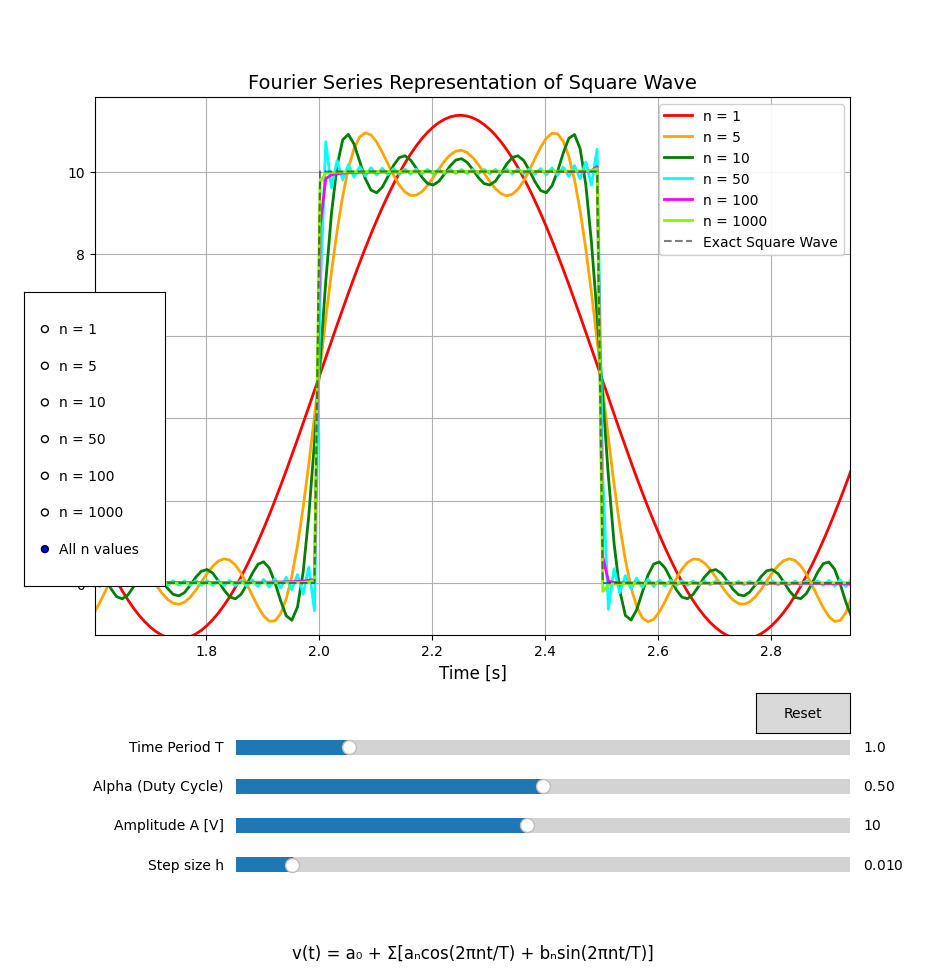
\includegraphics[width=1\linewidth]{figs/fourier convergence.png}
    
    \label{fig:enter-label}
\end{figure}


\chapter{Effect of Time Constant}
The time constant $\tau = \frac{L}{R}$ plays a crucial role in determining the circuit's response. We will use the concept of rise time and settling time to analyze, 
\begin{itemize}
    \item \textbf{Rise Time: } Time taken for the output to reach $90\%$ of its steady state value from $0$.
    \item \textbf{Settling Time: } Time taken for output to settle to $\pm 2\%$ of steady state value
\end{itemize}
We analyze three cases in detail:

\section{Case 1: $\tau \ll T$ (Small Time Constant)}
When the time constant is much smaller than the period of the square wave:

\begin{itemize}
    \item \textbf{Circuit Interpretation}: The circuit behaves similarly to a series RL circuit given a DC input. This is due to the high value of $T$ as compared to the time constant which allows the inductor to comfortably charge and discharge almost fully (Depends on $\alpha$ value also as the inductor might not fully charge or discharge for very low or very high values of $\alpha$) 
    \item \textbf{Rise Time}: Extremely short (approximately $3\tau$), as the current quickly approaches its steady-state value of $\frac{10}{R}$ during the ON period.
    \item \textbf{Settling Time}: Very short, typically around $4\tau$ to $5\tau$, meaning the current reaches steady state well before the square wave's value goes to $0$.
    \item \textbf{Mathematical Analysis}: For $\tau \ll T$, the transient term $e^{-\frac{t}{\tau}}$ in the expression for current decays rapidly. The current can be approximated as,\\     
    When the output of square wave is "HIGH", ( i.e. $0 < t < \alpha T$), this becomes:
    \begin{equation}
    i(t) \approx \frac{10}{R}(1 - e^{-\frac{t}{\tau}})
    \end{equation}
    
    When the output of square wave is "LOW" ( i.e. $\alpha T < t < T$). This expresssion is under the assumption that the inductor is almost fully charged, so initial current in inductor $i(t) \approx \frac{10}{R}$
    \begin{equation}
    i(t) \approx \frac{10}{R}e^{-\frac{(t-\alpha T)}{\tau}}
    \end{equation}
    This is very similar to the charging and discharging behaviour of a series RL circuit to DC input. \\
    $e^{-\frac{t}{\tau}}$ approaches zero quickly, the transient terms in the Fourier series expression disappear.
    \begin{align}
        i(t)  \approx \frac{10\alpha}{R} + \frac{10}{\alpha R} \sum_{n=1}^{\infty} \left(\frac{\sin ((2\pi \alpha - \omega_0 t)n)}{n}\right)
    \end{align}
    \item \textbf{Duty Ratio Effect}: The duty ratio $\alpha$ significantly affects the shape of the current waveform:\\
    Code used, \url{https://github.com/ArjunPavanje/EE1060/blob/main/Quiz3/codes/numerical_methods.py}
    \begin{itemize}
        \item For $\alpha \ll 0.5$, The inductor charges as much as possible during the limited time during which the input wave is $HIGH$, then it almost fully discharges (current goes to $0$) in the longer $LOW$ portion of input wave. This repeats for each cycle
        \pagebreak
        \begin{figure}[h!]
	   \centering
	   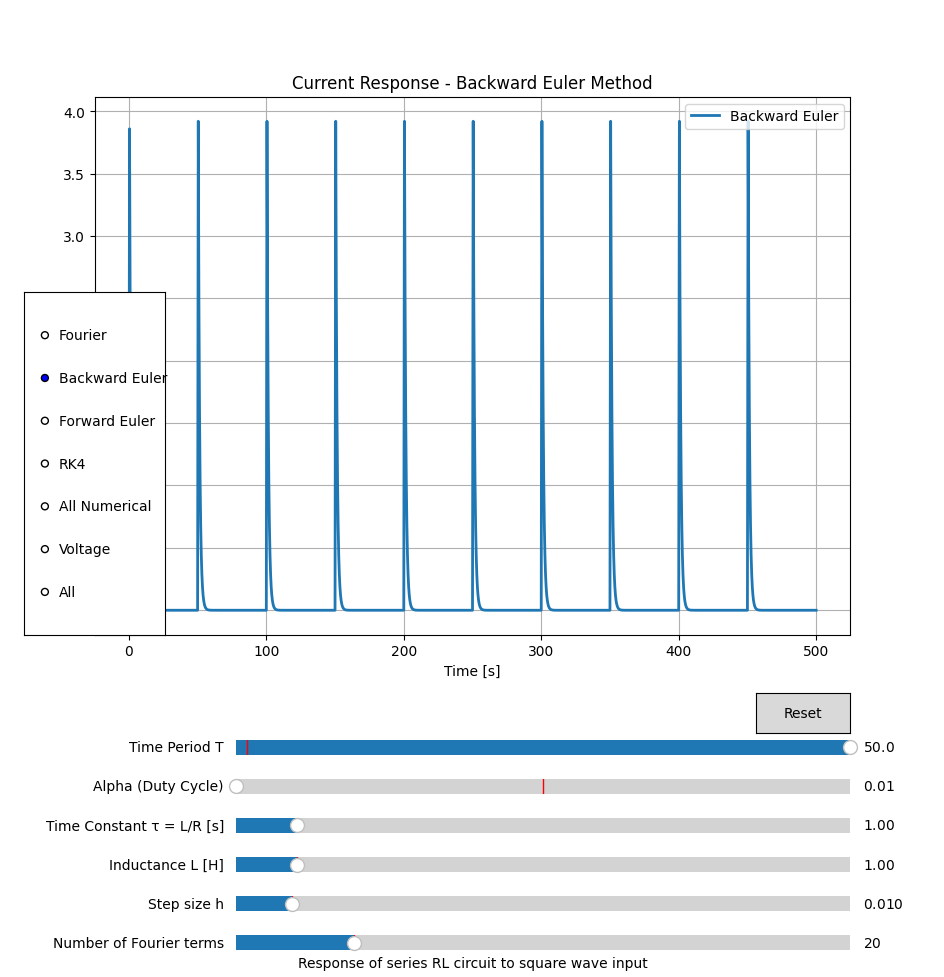
\includegraphics[scale=0.6]{figs/tau<<T-1.png}
        \end{figure}
        \item For $\alpha \approx 0.5$, the current waveform is symmetric. The inductor is capable of becoming fully charged and fully discharged in the $HIGH$ and $LOW$ portions of the input wave, respectively. 
        \pagebreak
        \begin{figure}[h!]
	   \centering
	   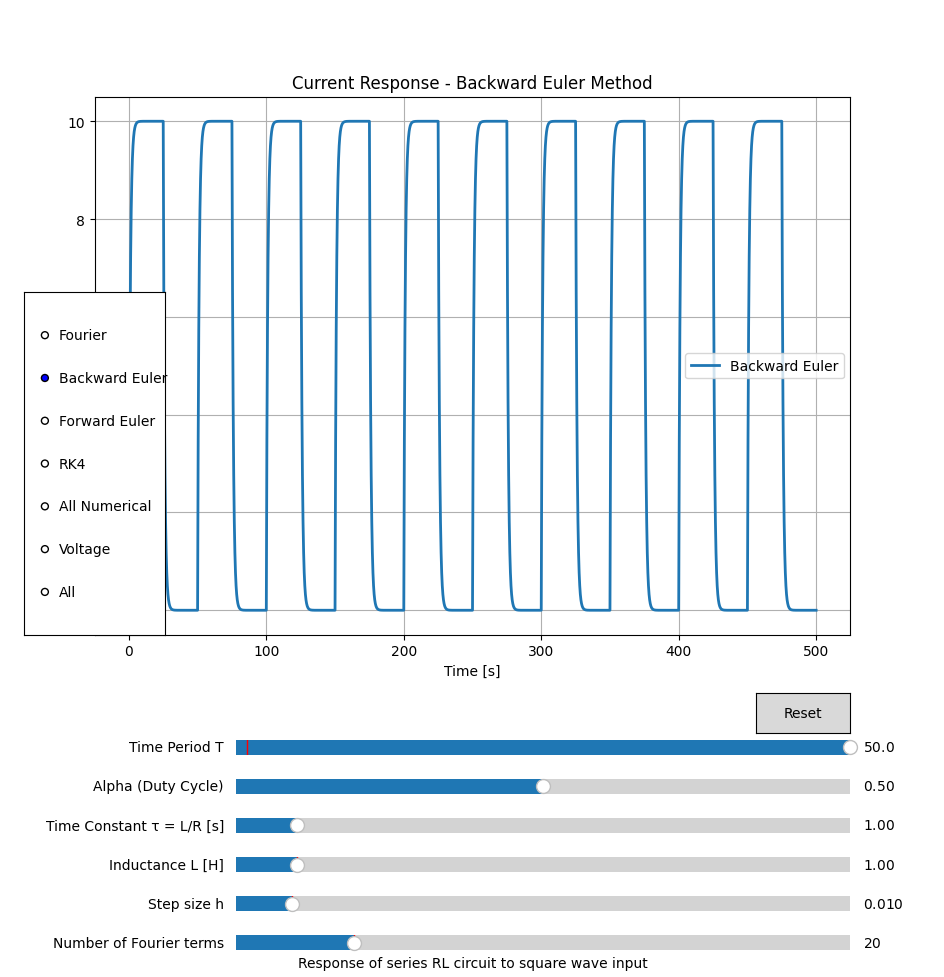
\includegraphics[scale=0.6]{figs/tau<<T-2.png}
        \end{figure} 
        
        \item For $\alpha \gg 0.5$, The inductor gets almost fully charged and reaches steady state (nearly) in the long duration for which input wave is $HIGH$. Due to the larger value of $\alpha$, the inductor discharges by a very little amount. This cycle repeats with the inductor starting with some amount of inital current from the second cycle onward.
        \pagebreak
        \begin{figure}[h!]
	   \centering
	   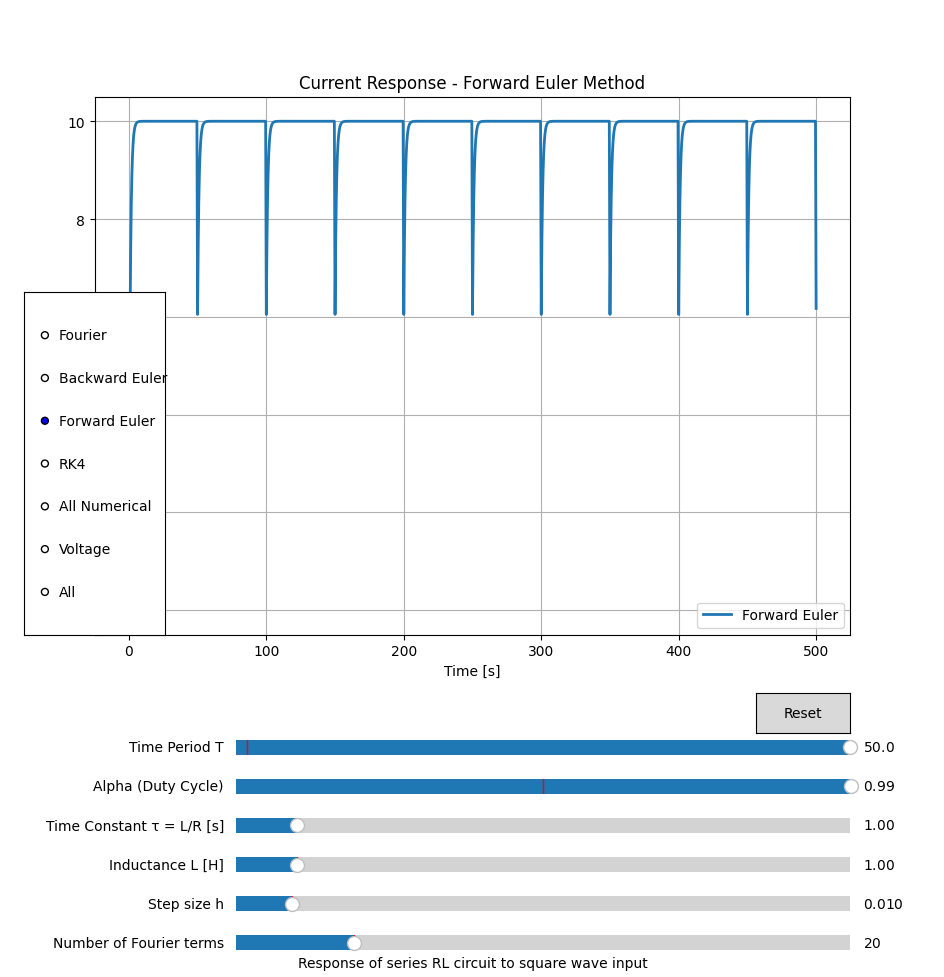
\includegraphics[scale=0.6]{figs/tau<<T-3.png}
        \end{figure}
    \end{itemize}
 
    To see the effect of changing $\alpha$, run the code above (To see the results clearly set $T$ to the maximum using slider and leave the other options unchanged) and use the slider to change $\alpha$ values.
    
\end{itemize}

\section{Case 2: $\tau \approx T$ (Comparable Time Constant)}
When the time constant is comparable to the period of the square wave:

\begin{itemize}
    \item \textbf{Physical Interpretation}: The inductor charges to some extent in the $HIGH$ period of square wave, then discharges to some extent. The extent of charging and discharging is governed by $\alpha$ value. Depending on $\alpha$ there will be three cases which are mentioned below.
    \item \textbf{Rise Time}: It is hard to comment on rise time as value of current in steady state oscillates a lot (so it is hard to calculate time taken to reach $90\%$ of its value)
    \item \textbf{Settling Time}: We can't comment on settling time as even in steady state, current oscillates a lot.
    \item \textbf{Mathematical Analysis}: For this case, no much simplification can be done, obtained expression (via fourier series or any numerical methods) must be used without approximation.
    
   \item \textbf{Duty Ratio Effect}: The duty ratio $\alpha$ significantly affects the shape of the current waveform:\\
   Code used, \url{https://github.com/ArjunPavanje/EE1060/blob/main/Quiz3/codes/numerical_methods.py}
    \begin{itemize}
        \item For $\alpha \ll 0.5$, Due to very small $\alpha$ value, inductor is charged very very less.
        \begin{figure}[h!]
	\centering
	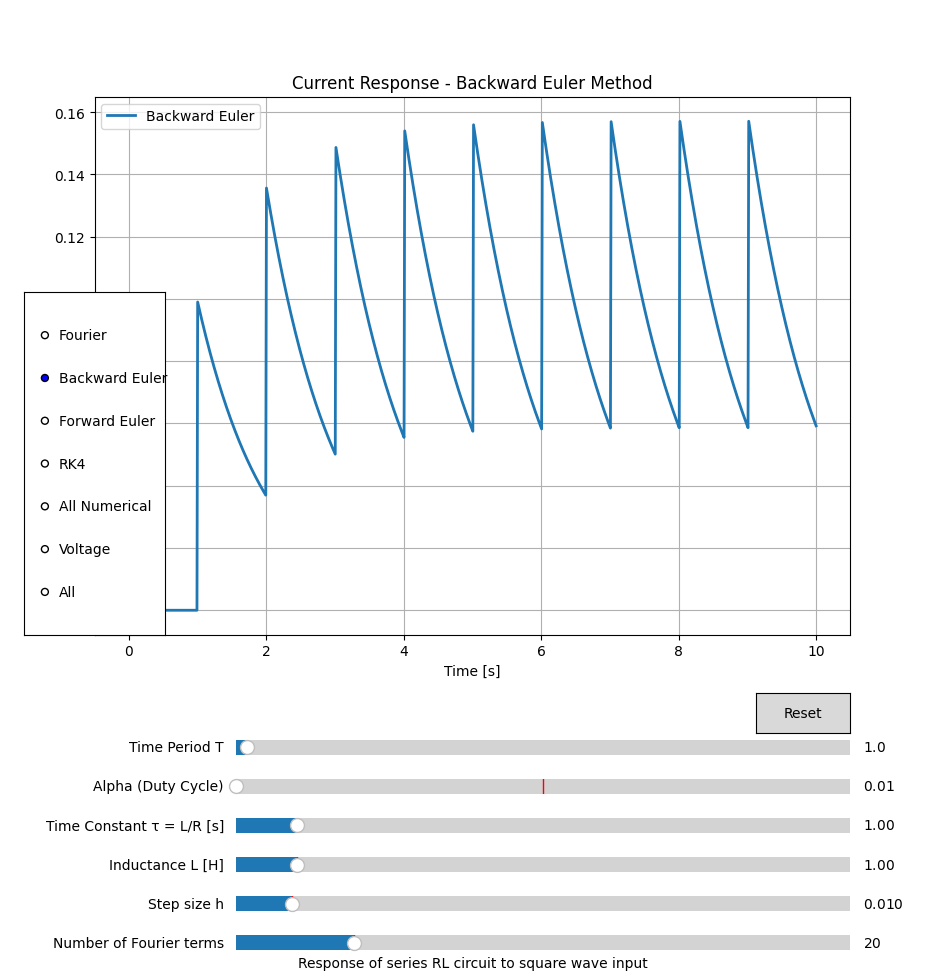
\includegraphics[scale=0.4]{figs/tau=T-1.png}
        \end{figure}
        \item For $\alpha \approx 0.5$, for the first few cycles, the inductor gets charged to some extent when the input wave is $HIGH$, but when it is $LOW$ it doesn't fully discharge, i.e. when it goes into the next half cycle it still has some initial current. The current waveform is approximately symmetric at steady state (it charges by some ammount in the first $\alpha T$ seconds of cycle, and discharges by the same amount in the remaining time in the cycle).
        \begin{figure}[h!]
	\centering
	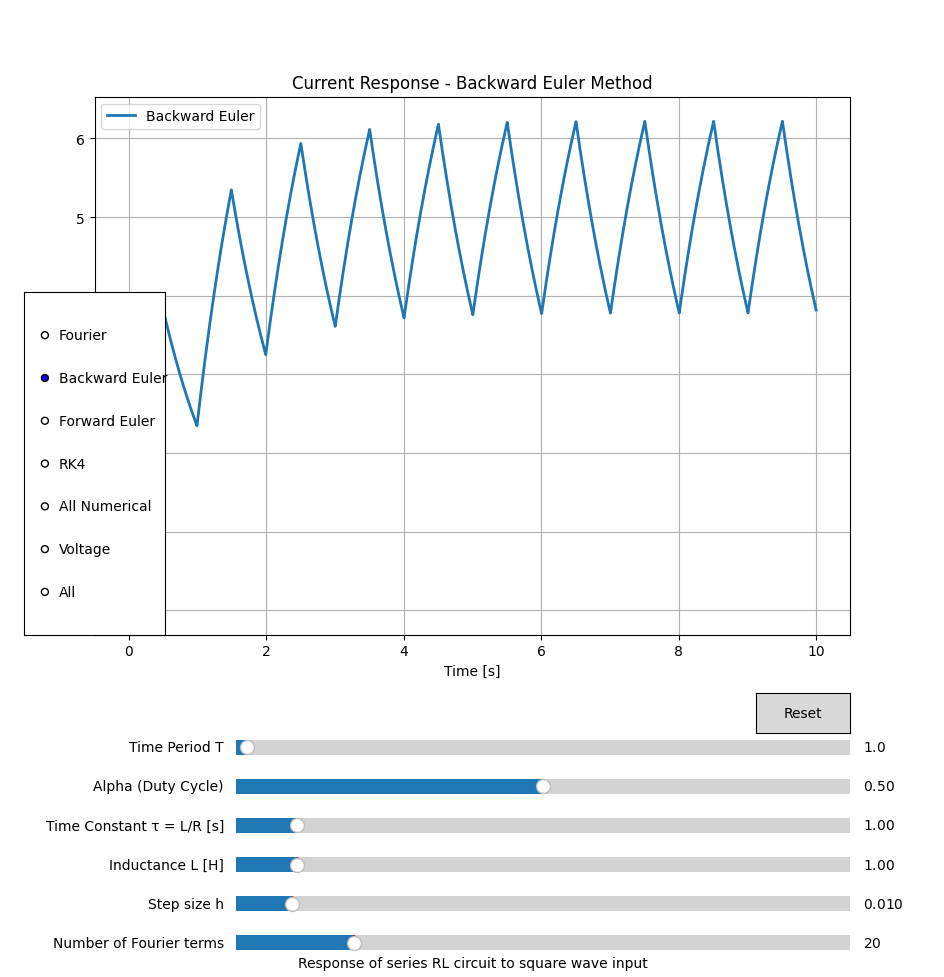
\includegraphics[scale=0.6]{figs/tau=T-2.png}
        \end{figure}
    
        \item For $\alpha \gg 0.5$, Due to very high $\alpha$ value, the graph tends to that of a series RL circuit under DC input as the square wave input is nearly DC as $\alpha \rightarrow 1$. This case for $\tau \ll T$, does not tend to a similar graph as more discharging happens to a lower value of $\tau$. A lower value $\tau$ implies both faster charging and discharging. 
        \begin{figure}[h!]
	\centering
	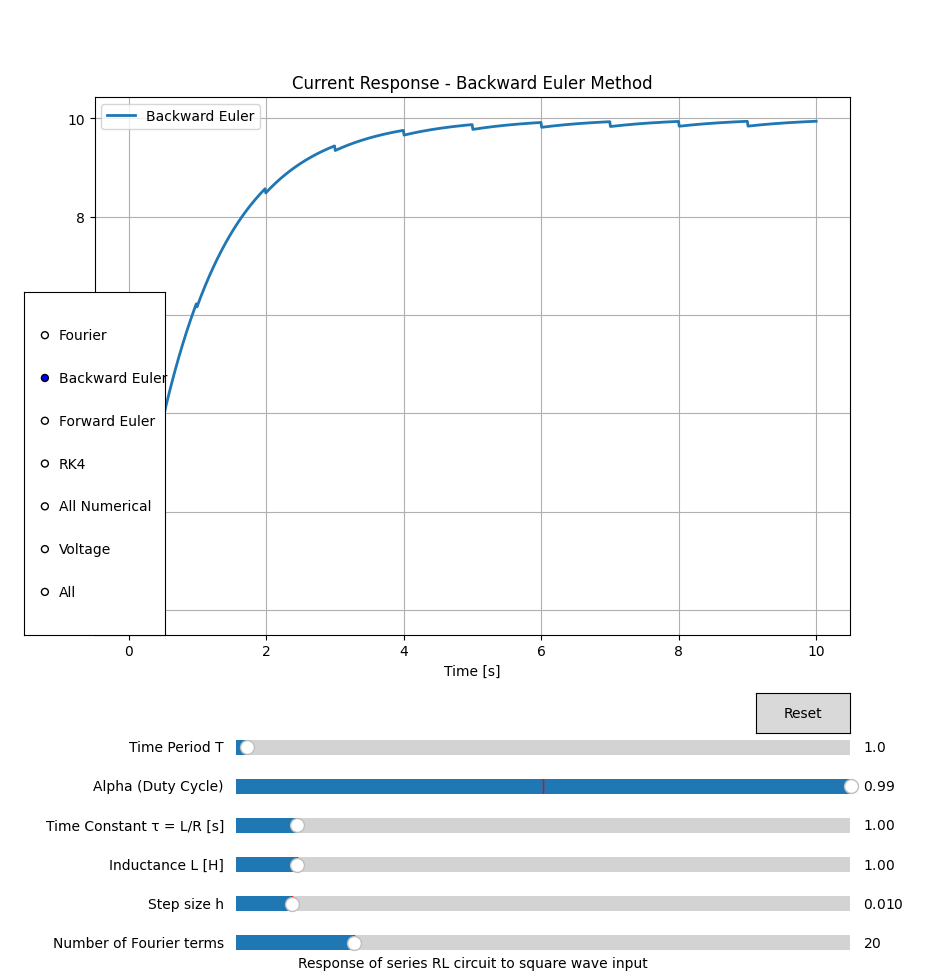
\includegraphics[scale=0.6]{figs/tau=T-3.png}
        \end{figure}
    \end{itemize}
    To see the effect of changing $\alpha$, run the code below (In the code, $\tau = T = 1$, so no need to adjust $\tau, T$ manually, just select a numerical method) and use the slider to change $\alpha$ values.
\end{itemize}

\section{Case 3: $\tau \gg T$ (Large Time Constant)}
When the time constant is much larger than the period of the square wave:

\begin{itemize}
    \item \textbf{Physical Interpretation}: Due to the relatively larger value of time constant as compared to time period of the wave, charging and discharging happen extremely slowly
    \item \textbf{Rise Time}: Very long, much longer than the period of the square wave. The current never approaches the theoretical steady-state value.
    \item \textbf{Settling Time}: Much longer than the period, typically on the order of $4\tau$ to $5\tau$, which spans multiple cycles of the input.
    \item \textbf{Mathematical Analysis}: Waveforms tend to be more and more triangular as higher $\tau$ value implies slower charging and discharging. In the fourier series, we can put $\frac{1}{\tau} \rightarrow 0$, we get 
    \begin{align}
    i(t) \approx \frac{10}{\pi \omega_0 L} \sum_{n=1}^{\infty} \frac{\cos(2\pi \alpha - \omega_0 t)n)}{n^2}
    \end{align}
    \item \textbf{Duty Ratio Effect: } The duty ratio $\alpha$ significantly affects the shape of the current waveform:\\
    Code used, \url{https://github.com/ArjunPavanje/EE1060/blob/main/Quiz3/codes/numerical_methods.py}
    \begin{itemize}
        \item For $\alpha \ll 0.5$, Inductor charges very little due to the small $\alpha$ value, but discharges even slower and lesser in the next half cycle (due to relatively high $\tau$ value) so inducotr doesn't fully discharge.
        \pagebreak
        \begin{figure}[h!]
	\centering
	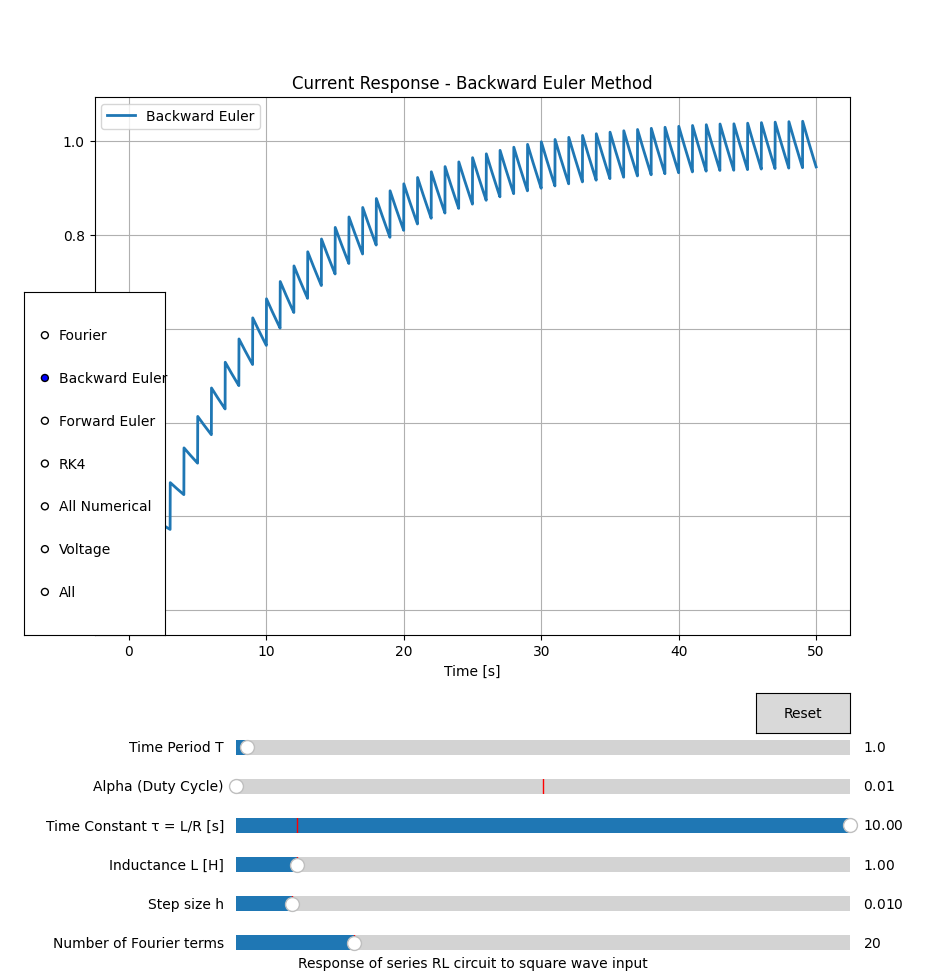
\includegraphics[scale=0.6]{figs/tau>>T-1.png}
        \end{figure}
        \item For $\alpha \approx 0.5$, inductor charges for half the cycle, discharges in the other half. Extent of charging is slightly more, so going into the next cycle, the inductor starts with more current. In steady state, the inductor charges and discharges in nearly equal amounts in a cycle
        \pagebreak
        \begin{figure}[h!]
	\centering
	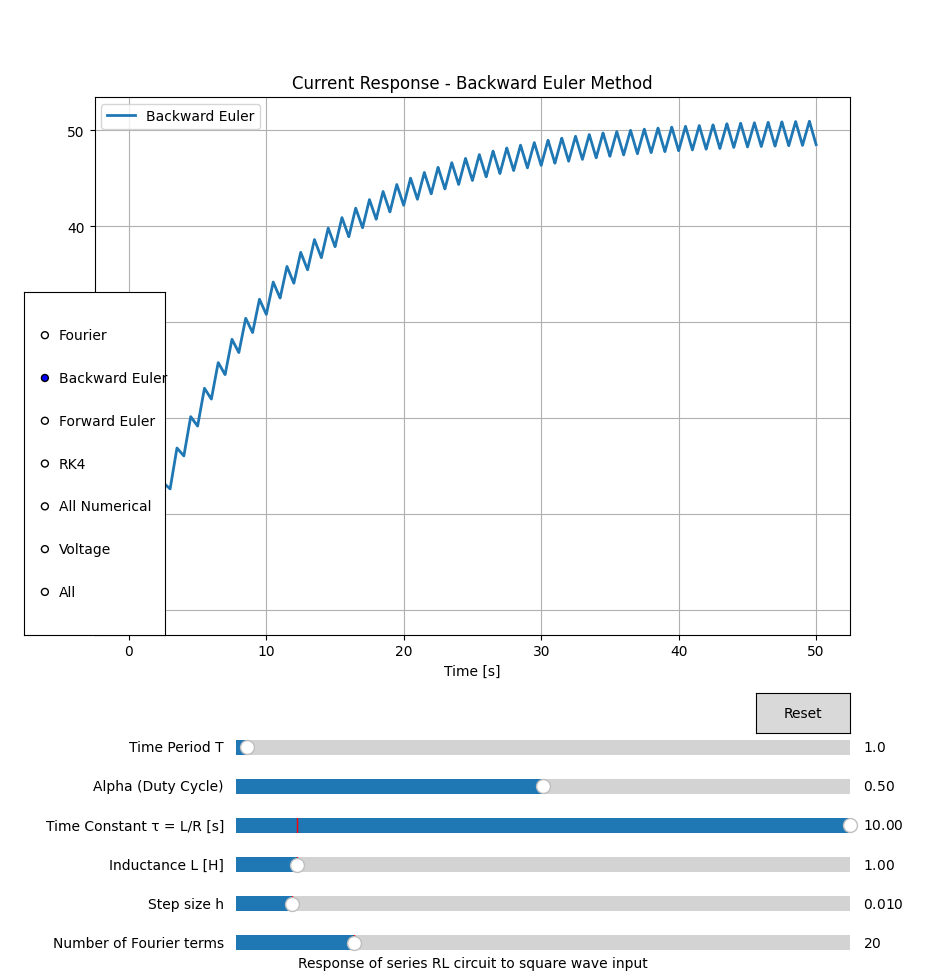
\includegraphics[scale=0.6]{figs/tau>>T-2.png}
        \end{figure}
    
        \item For $\alpha \gg 0.5$, similar to this case for $\tau \approx T$, current output will tend to (even more so than in the previous case) the output of a series RL circuit to DC input (due to very low $\alpha$ value which makes input square wave nearly DC). Due to higher $\tau, \alpha$ values, it discharges even lesser.
        \pagebreak
        \begin{figure}[h!]
	\centering
	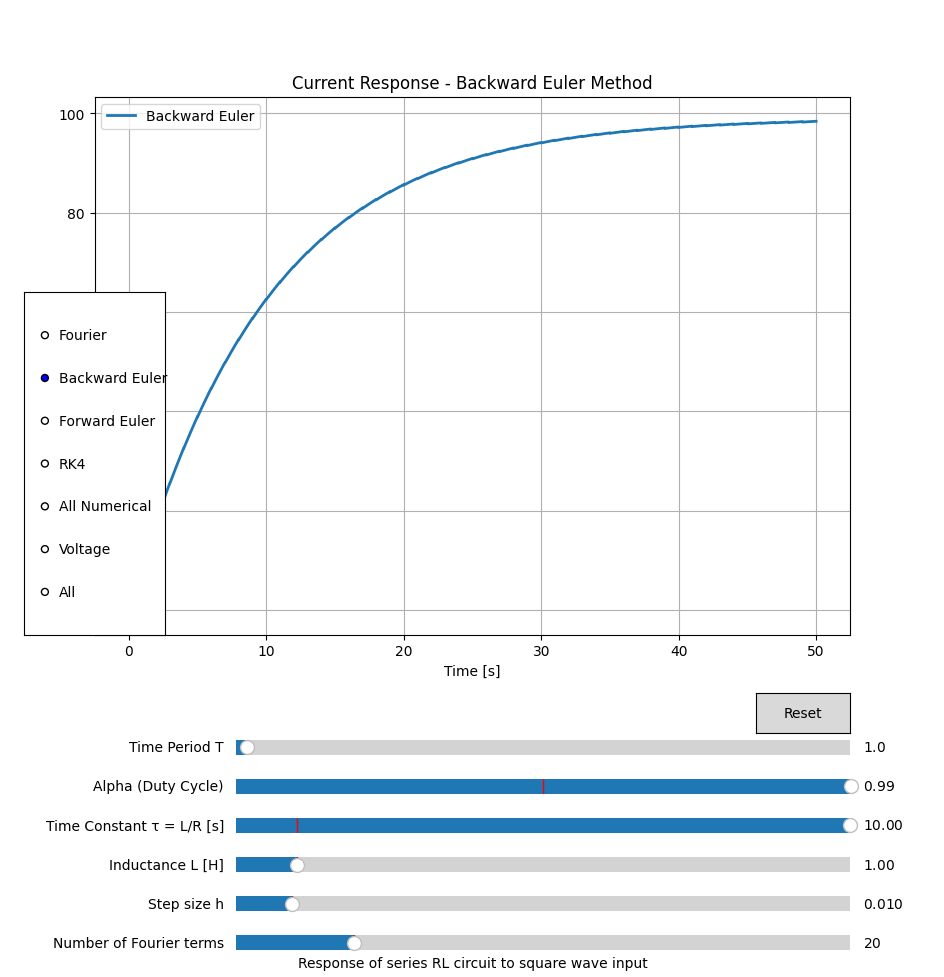
\includegraphics[scale=0.6]{figs/tau>>T-3.png}
        \end{figure}
    \end{itemize}
    To see the effect of changing $\alpha$, run the code below (In the code set $\tau$ to the maximum using the slider, just select a numerical method) and use the slider to change $\alpha$ values. It is also recommended to increase number of cycles of wave plotting while seeing this.
\end{itemize}
\chapter{Error analysis}
\section{Forward Euler}
The error in the \textbf{Forward Euler method} can be analyzed using a \textbf{Taylor series expansion}. Given a general differential equation:
\begin{align}
    \frac{dy}{dt}=f(t,y)
\end{align}
with an exact solution y(t), we expand it around $t_{n}$ using the Taylor series:
\begin{align}
    y(t_{n+1})=y(t_{n})+h\frac{dy}{dt}\Big|_{t_n}+\frac{h^2}{2}\frac{d^2y}{dt^2}\Big|_{t_n}+O(h^3)
\end{align}
Substituting the differential equation $\frac{dy}{dt}=f(t,y)$ and using the Euler approximation:
\begin{align}
    y_{n+1}=y_{n}+hf(t_{n},y_{n})
\end{align}
The local truncation error is given by the omitted higher-order terms:
\begin{align}
    E_{n}=\frac{h^2}{2}\frac{d^2y}{dt^2}+O(h^3)
\end{align}
\section{Backward Euler}
The error in the \textbf{Backward Euler} method can also be analyzed using a \textbf{Taylor series expansion}.  

Given the general differential equation:  
\begin{equation}
\frac{dy}{dt} = f(t, y)
\end{equation}

with an exact solution $ y(t) $, we expand it around $ t_{n+1} $ using the Taylor series:  

\begin{equation}
y(t_n) = y(t_{n+1}) + h \frac{dy}{dt} \bigg|_{t_{n+1}} + \frac{h^2}{2} \frac{d^2y}{dt^2} \bigg|_{t_{n+1}} + O(h^3)
\end{equation}

Using the \textbf{Backward Euler} approximation:

\begin{equation}
y_{n+1} = y_n + h f(t_{n+1}, y_{n+1})
\end{equation}

The \textbf{local truncation error} is given by the neglected higher-order terms:

\begin{equation}
E_n = \frac{h^2}{2} \frac{d^2y}{dt^2} \bigg|_{t_{n+1}} + O(h^3)
\end{equation}

Since the error term structure is similar to Forward Euler, \textbf{Backward Euler is also first-order accurate}, but it provides better stability for stiff systems.
\section{Runge-Kutta 4th Order (RK4)}
The \textbf{Runge-Kutta 4th order (RK4)} method provides a higher-order approximation to the solution of the differential equation:

\begin{equation}
\frac{dy}{dt} = f(t, y)
\end{equation}

Using Taylor series expansion, the exact solution at $ t_{n+1} $ is given by:

\begin{equation}
y(t_{n+1}) = y(t_n) + h \frac{dy}{dt} \Big|_{t_n} + \frac{h^2}{2} \frac{d^2y}{dt^2} \Big|_{t_n} + \frac{h^3}{6} \frac{d^3y}{dt^3} \Big|_{t_n} + \frac{h^4}{24} \frac{d^4y}{dt^4} \Big|_{t_n} + O(h^5)
\end{equation}

The RK4 method approximates the solution using intermediate function evaluations:

\begin{align}
k_1 &= hf(t_n, y_n) \\
k_2 &= hf\left(t_n + \frac{h}{2}, y_n + \frac{h}{2} k_1 \right) \\
k_3 &= hf\left(t_n + \frac{h}{2}, y_n + \frac{h}{2} k_2 \right) \\
k_4 &= hf(t_n + h, y_n + h k_3)
\end{align}

The next-step approximation is given by:

\begin{equation}
y_{n+1} = y_n + \frac{1}{6} (k_1 + 2k_2 + 2k_3 + k_4)
\end{equation}

The \textbf{local truncation error} for RK4 is derived from the omitted higher-order terms:

\begin{equation}
E_n = \frac{h^5}{120} \frac{d^5y}{dt^5} + O(h^6)
\end{equation}

This indicates that the RK4 method is \textbf{fourth-order accurate}, meaning the global error scales as $ O(h^4) $, making it significantly more accurate than both Forward and Backward Euler methods for the same step size $ h $.\\

Relative Errors of each method can be compared in the image below,
\begin{figure}[h!]
\centering
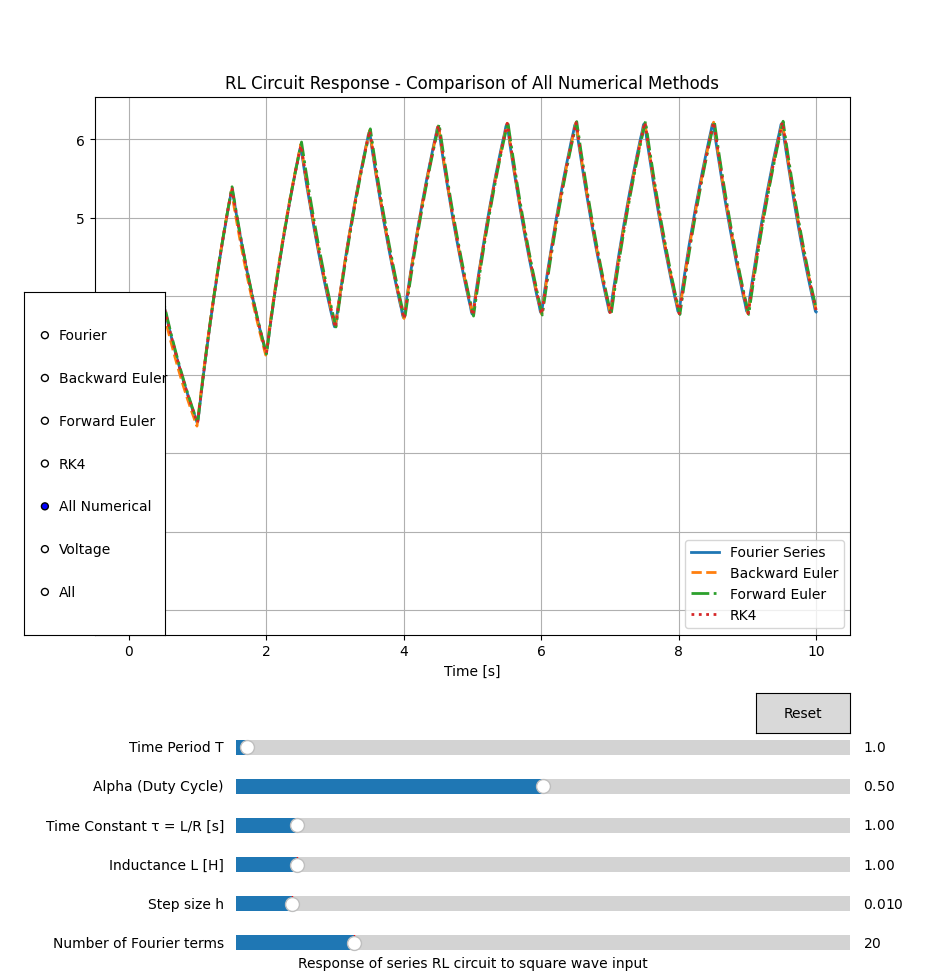
\includegraphics[scale=0.5]{figs/numerical-1.png}
\end{figure}

\begin{figure}[h!]
\centering
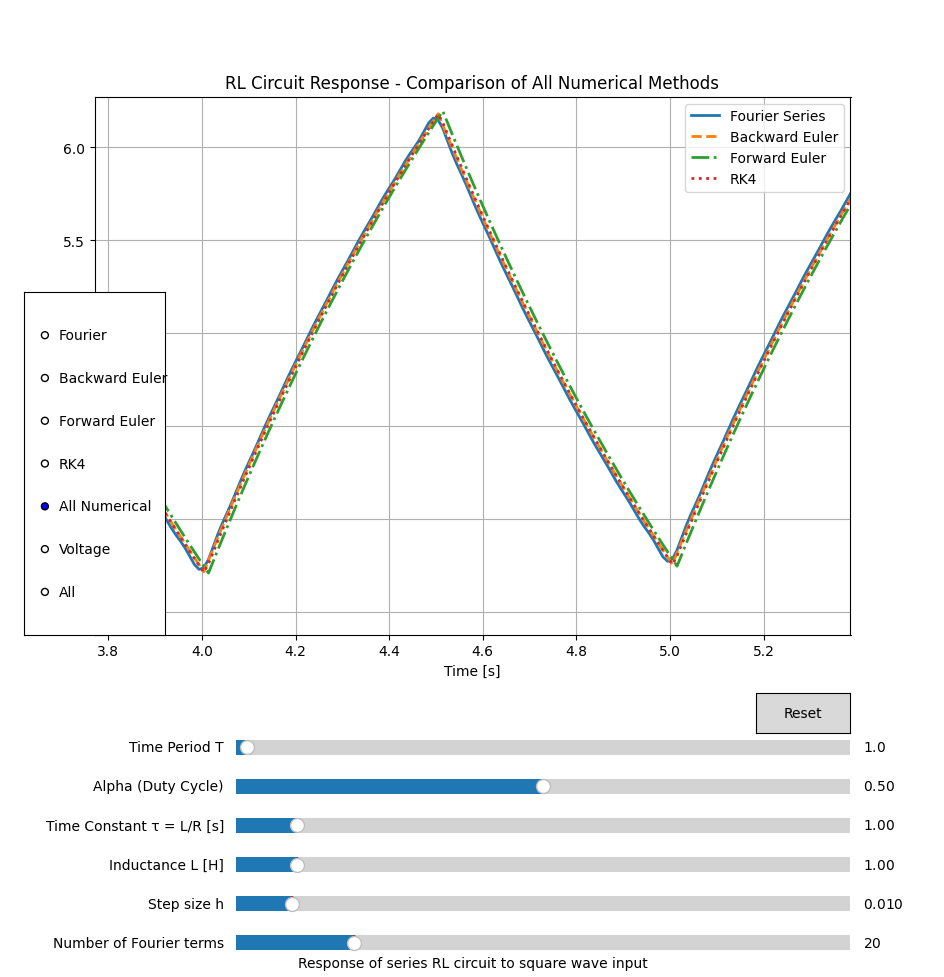
\includegraphics[scale=0.5]{figs/numerical-2.png}
\end{figure}

\begin{figure}[h!]
\centering
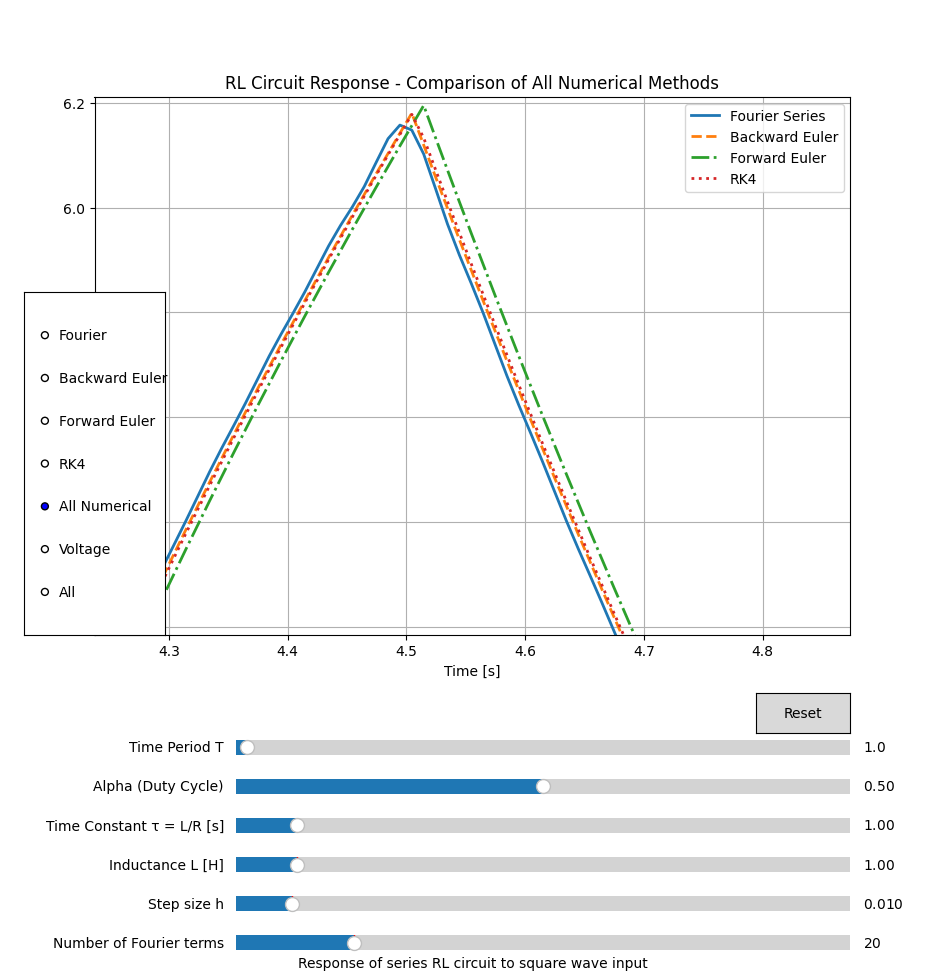
\includegraphics[scale=0.5]{figs/numerical-3.png}
\end{figure}
Code used, \url{https://github.com/ArjunPavanje/EE1060/blob/main/Quiz3/codes/numerical_methods.py}


\chapter{Detailed Analysis of Step Size and Stability}

\section{Forward Euler Method Stability}
The stability of the Forward Euler method depends critically on the step size $h$ in relation to the time constant $\tau$.

\textbf{Stability Condition Derivation:}
For the RL circuit, the Forward Euler update equation is:
\begin{equation}
i_{n+1} = i_n + h \cdot \frac{v(t_n) - Ri_n}{L}
\end{equation}

For stability analysis, we consider the homogeneous part (setting $v(t_n) = 0$):
\begin{equation}
i_{n+1} = i_n - h \cdot \frac{Ri_n}{L} = i_n(1 - \frac{hR}{L})
\end{equation}

For stability, we require $|1 - \frac{hR}{L}| < 1$, which gives:
\begin{equation}
-1 < 1 - \frac{hR}{L} < 1
\end{equation}

The right inequality gives $\frac{hR}{L} < 2$, or $h < \frac{2L}{R} = 2\tau$. The left inequality gives $\frac{hR}{L} < 2$, which is the same constraint.

Therefore, the stability condition is:
\begin{equation}
h < 2\tau = \frac{2L}{R}
\end{equation}

\textbf{Practical Implications:}
\begin{itemize}
    \item For $\tau = 0.1$ (e.g., $L = 0.1$H, $R = 1\Omega$), the step size must be $h < 0.2$ for stability.
    \item For $\tau = 1$ (e.g., $L = 1$H, $R = 1\Omega$), the step size must be $h < 2$ for stability.
    \item For $\tau = 10$ (e.g., $L = 10$H, $R = 1\Omega$), the step size must be $h < 20$ for stability.
\end{itemize}

\textbf{Experimental Verification:}
\begin{figure}[h!]
\centering
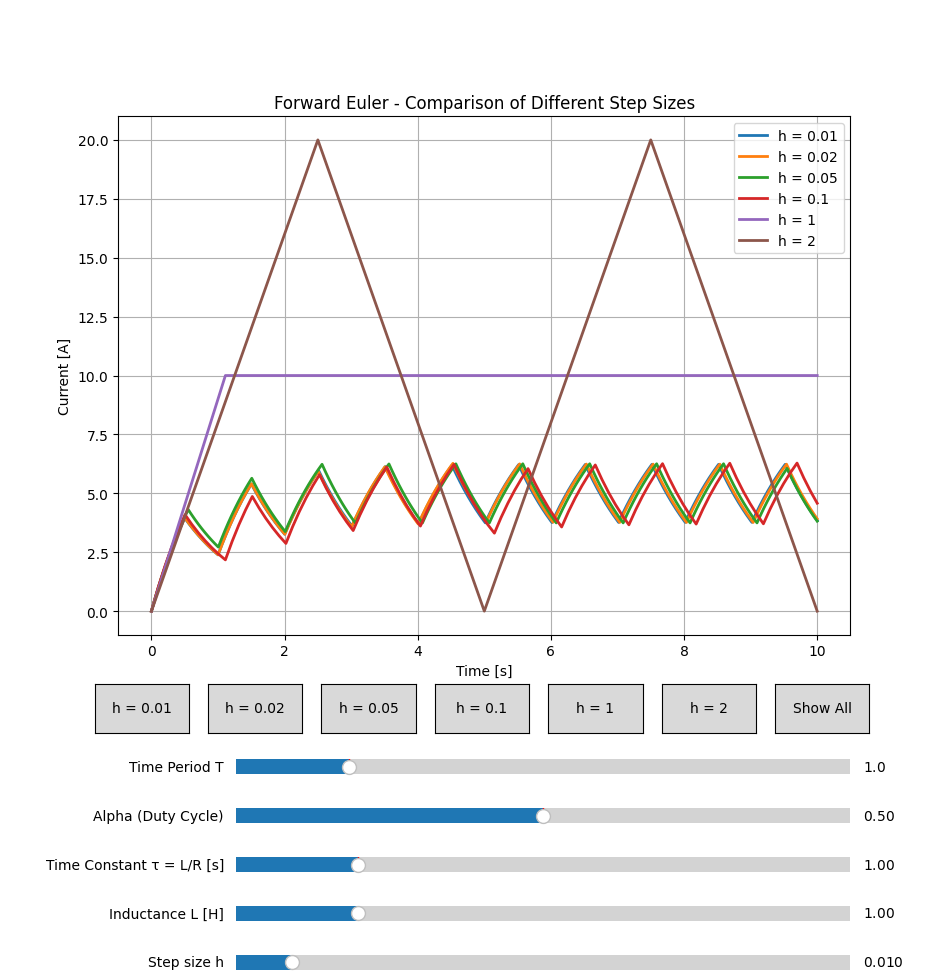
\includegraphics[scale=0.5]{figs/forward_euler_stability.png}
\end{figure}
From the error analysis table(for R=1$\Omega$ ,L=1H, T=1sec, $\alpha$=0.5)  we observe:
\begin{table}[H]
\centering
\begin{tabular}{|c|c|c|}
\hline
h value & Deviation in 1st step & Deviation in 2nd step \\
\hline
0.01 & 0.000498 & 0.000986 \\
\hline
0.1 & 0.048 & 0.087 \\
\hline
0.4 & 0.7032 & -0.5149 \\
\hline
\end{tabular}
\caption{Error in Forward Euler method for different step sizes}
\end{table}

The negative deviation in the second step for $h = 0.4$ indicates oscillatory behavior, which is a sign of approaching instability. As $h$ increases further beyond $2\tau$, the solution would become completely unstable.

\section{Backward Euler Method Stability}
The Backward Euler method is unconditionally stable for any step size, which is a significant advantage for stiff systems.

\textbf{Stability Analysis:}
For the RL circuit, the Backward Euler update equation is:
\begin{equation}
i_{n+1} = \frac{Li_n + hv(t_{n+1})}{L + hR} = \frac{i_n\tau + hv(t_{n+1})}{\tau + h}
\end{equation}

For stability analysis, we consider the homogeneous part (setting $v(t_{n+1}) = 0$):
\begin{equation}
i_{n+1} = \frac{i_n\tau}{\tau + h}
\end{equation}

Since $\tau > 0$ and $h > 0$, we have $0 < \frac{\tau}{\tau + h} < 1$ for all positive values of $h$. This means that the magnitude of the amplification factor is always less than 1, ensuring unconditional stability regardless of the step size.
\begin{figure}[h!]
\centering
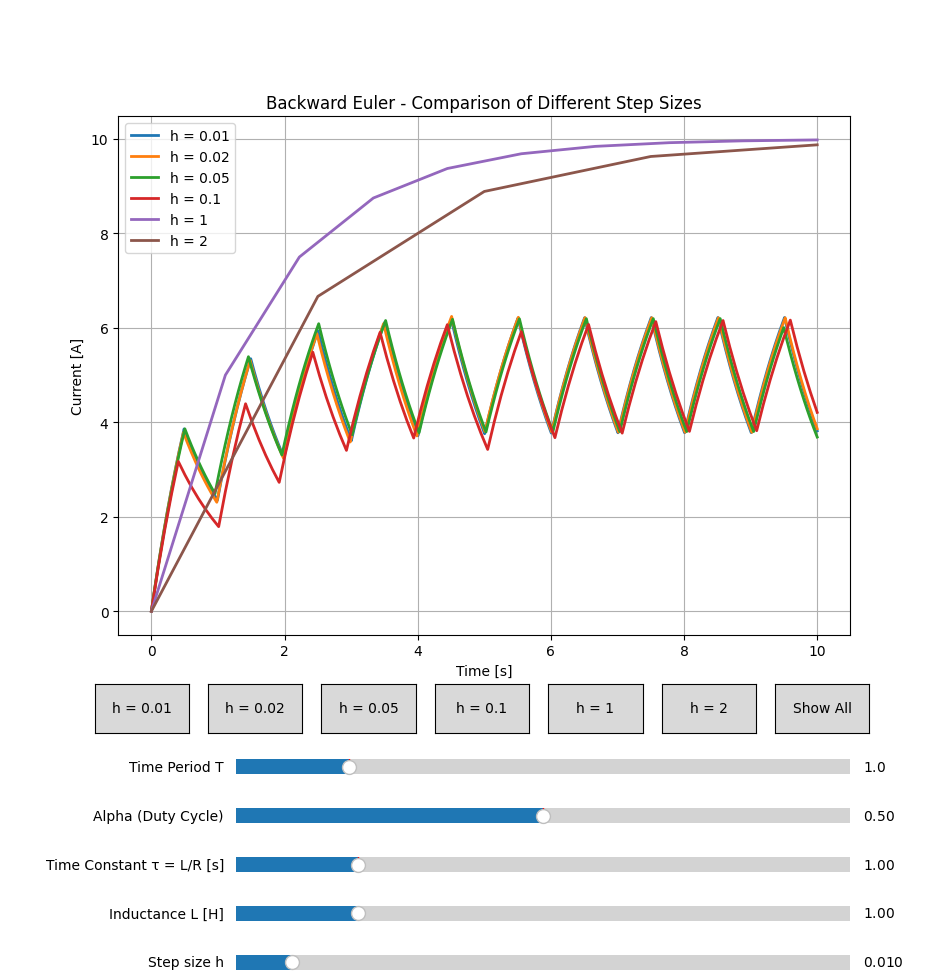
\includegraphics[scale=0.4]{figs/backward_euler_stability.png}
\end{figure}

\textbf{Practical Implications:}
\begin{itemize}
    \item The Backward Euler method allows for larger step sizes without stability issues, making it suitable for stiff systems where $\tau$ is very small.
    \item However, larger step sizes still lead to reduced accuracy, even though stability is maintained.
    \item The method introduces numerical damping, which can be beneficial for suppressing non-physical oscillations but may lead to overdamped solutions.
\end{itemize}

\section{RK4 Method Stability}
The RK4 method has a much larger stability region than Forward Euler, but it is still conditionally stable.

\textbf{Stability Region:}
For linear systems, the stability region of RK4 extends to approximately $h < 2.78\tau$, which is about 39\% larger than Forward Euler's stability region.

\textbf{Practical Implications:}
\begin{itemize}
    \item RK4 allows for larger step sizes than Forward Euler while maintaining stability.
    \item The method's higher order of accuracy means that even with the same step size, RK4 produces much smaller errors than both Forward and Backward Euler methods.
    \item For the RL circuit with $\tau = 1$, RK4 remains stable for step sizes up to approximately $h = 2.78$, compared to $h = 2$ for Forward Euler.
\end{itemize}
\pagebreak
\begin{figure}[h!]
\centering
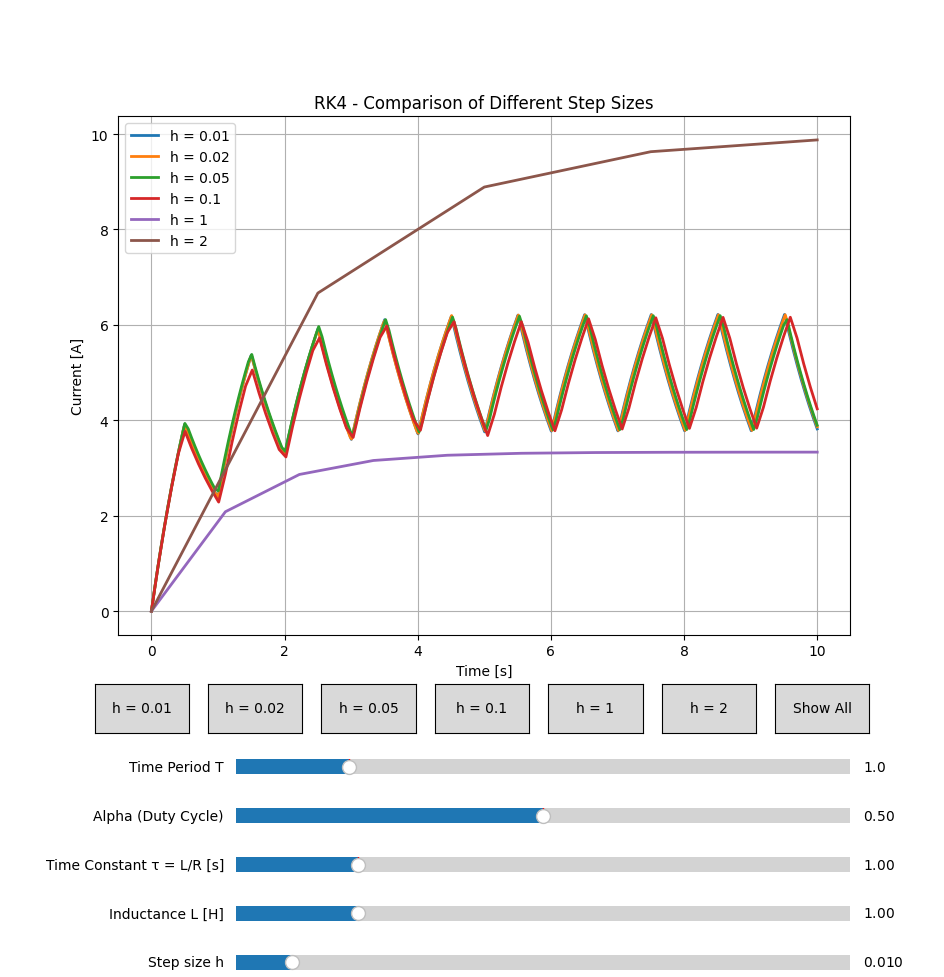
\includegraphics[scale=0.6]{figs/rk4_stability.png}
\end{figure}
All codes used for plotting may be found here, \url{https://github.com/ArjunPavanje/EE1060/tree/main/Quiz3/codes/stability}.
\section{Fourier Series}
Below is a code that shows how increasing number of coeffecients changes the plot.
\begin{figure}
    \centering
    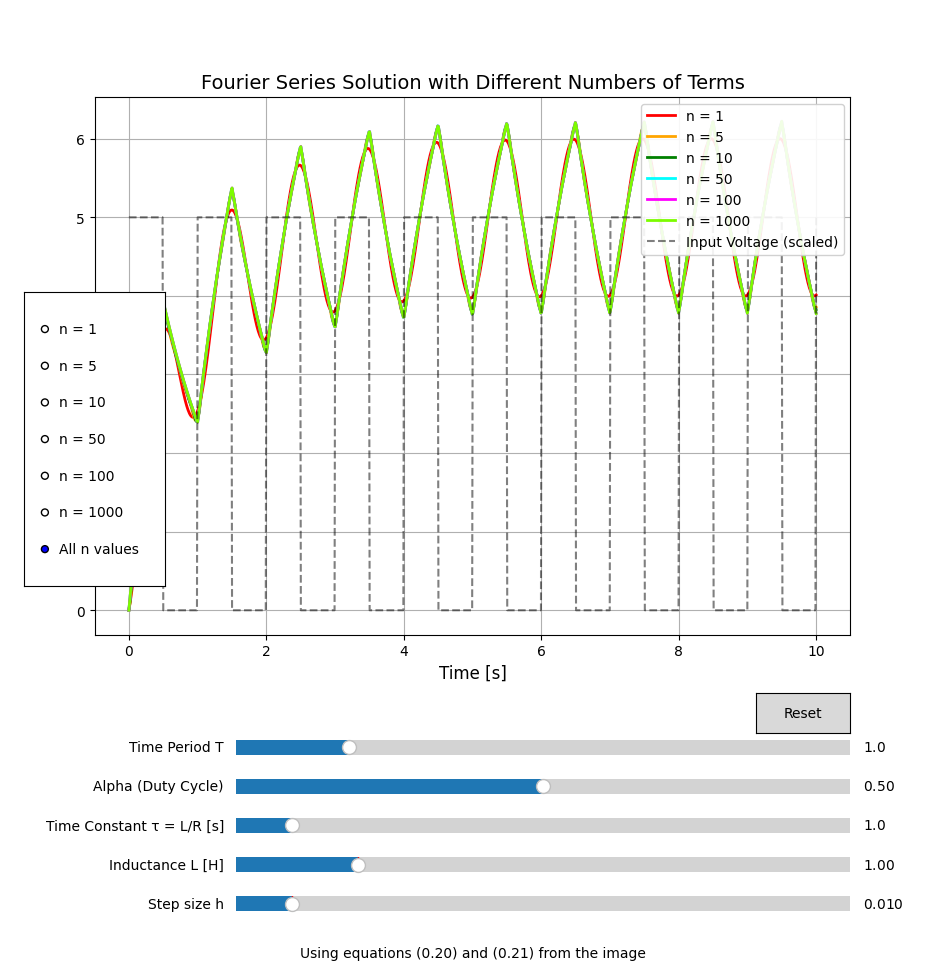
\includegraphics[width=1\linewidth]{figs/conv-1.png}
    \label{fig:enter-label}
\end{figure}
\begin{figure}
    \centering
    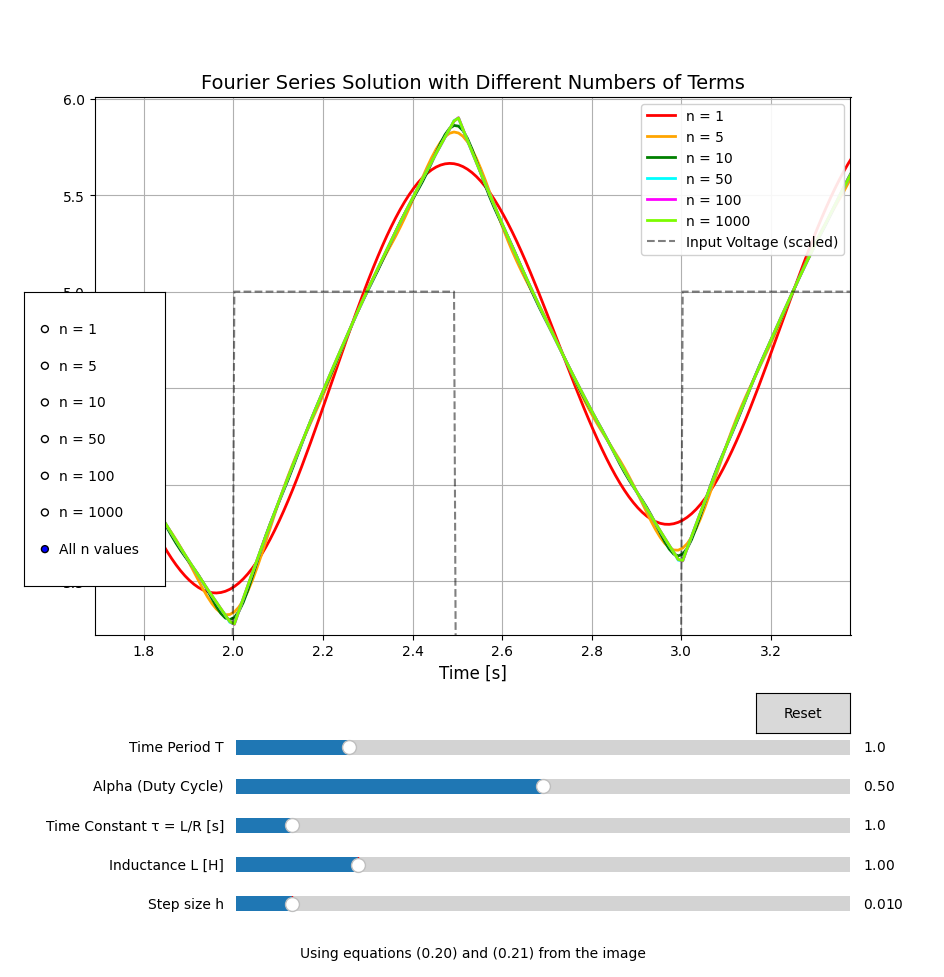
\includegraphics[width=1\linewidth]{figs/conv-2.png}
    \label{fig:enter-label}
\end{figure}
\begin{figure}
    \centering
    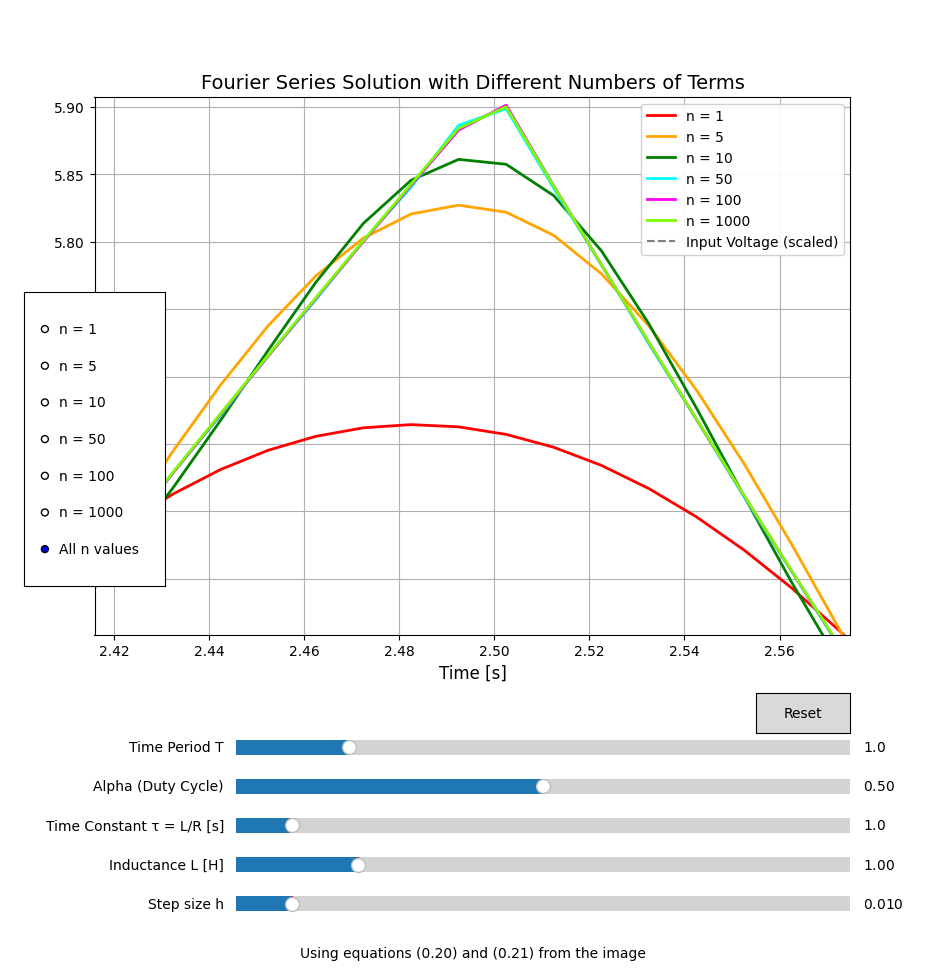
\includegraphics[width=1\linewidth]{figs/conv-3.png}
    \label{fig:enter-label}
\end{figure}
\url{https://github.com/ArjunPavanje/EE1060/blob/main/Quiz3/codes/fourier_convergence.py}
\chapter{Conclusion}

In this comprehensive study, we have systematically analyzed the response of a series RL circuit to a square wave input using both \textbf{numerical methods} (Forward Euler, Backward Euler, and Runge-Kutta 4th Order) and \textbf{analytical techniques} (Fourier series). By combining these approaches, we gained a \textbf{deeper understanding} of how the circuit responds under varying conditions, including changes in time constants and duty cycles.

\subsection{Key Insights}

\begin{itemize}
    \item \textbf{Numerical Methods:} Each numerical technique provided a different perspective on the circuit's transient behavior. \textbf{Forward Euler} demonstrated stability limitations, \textbf{Backward Euler} showed numerical damping effects, and \textbf{RK4} emerged as the most accurate due to its higher-order precision.
    
    \item \textbf{Fourier Series Analysis:} By representing the square wave input in the frequency domain, we observed how the circuit selectively attenuates higher-order harmonics, with the response heavily dependent on the circuit’s \textbf{time constant} and the \textbf{duty cycle} of the input signal.
    
    \item \textbf{Effect of the Time Constant} (\( \tau = L/R \)): A \textbf{small} \( \tau \) resulted in the circuit quickly following the input, while a \textbf{large} \( \tau \) caused a slower response, effectively acting as a low-pass filter.
    
    \item \textbf{Gibbs Phenomenon:} The presence of overshoot at discontinuities in the Fourier representation underscored the \textbf{limitations of truncated series approximations}, emphasizing the need for careful term selection in practical applications.
\end{itemize}

\subsection{Broader Implications \& Future Directions}

The insights from this study are highly relevant for \textbf{designing circuits in digital electronics, power systems, and signal processing applications}, where square wave inputs are common. Understanding the \textbf{trade-offs between numerical accuracy, stability, and computational cost} is essential for engineers working with transient responses.

Future work could involve exploring \textbf{nonlinear circuit elements, higher-order systems}, or even \textbf{adaptive numerical techniques} for improved efficiency. Additionally, extending this analysis to \textbf{real-world applications} such as filtering, modulation, and waveform shaping could provide deeper insights into practical circuit behavior.

Ultimately, this study highlights the power of \textbf{combining numerical and analytical techniques} to gain a more complete understanding of electrical systems, bridging the gap between \textbf{theory, computation, and real-world application}.

\end{document}

